\chapter{Modeling}
\label{sec:modeling}
The position controller proposed in this project will be model based. Therefore we need to define a detailed system which is to be controlled.

In this section the MAV system is stated. It starts by describing the multirotor platform. Then the equations of motion are derived for both translation and rotation. Additionally we include wind into the model. In the fourth part a system identification approach is described to approximate the attitude dynamics. Next the overall dynamics to be controlled are summarized in a system diagram. Finally the system is linearized.

In this project a cascaded control approach is chosen (see figure ). Attitude and motor control run at a high rate ($1000 \si{\hertz}$) in an inner loop, while the high level position controller runs at $100 \si{\hertz}$ in an outer loop. This decoupling is possible because the translational dynamics are much slower than the rotational dynamics. It simplifies the design of the position controller as only translational dynamics have to be considered explicitly and position control reduces to controlling the vehicles desired thrust and direction. 

In order for the vehicle to move to a reference position, the position controller computes the desired thrust force and roll, pitch, yaw angles. The inner loop then takes care of finding the appropriate moment applied to the vehicle body to archive the desired attitude. The attitude controller is given and its dynamics are identified as a linear system.

\begin{figure}
\centering
\includegraphics{images/controller_sketch.tikz}
\caption{Cascaded control sketch}
\label{pics:controller_sketch}
\end{figure}





Also we only consider translational dynamics as they are crucial for position control. The rotational dynamics are handled by the attitude controller. We approximate the closed loop attitude control with a linear system identification.

%%%%%%%%%%%%%%%%%%%%%%%%%%%%%%%%%%%%%%%%%%%%%%%%%%%%%%%%%%%%%%%%%%%%%%%%%%%%%%%
% Platform
%%%%%%%%%%%%%%%%%%%%%%%%%%%%%%%%%%%%%%%%%%%%%%%%%%%%%%%%%%%%%%%%%%%%%%%%%%%%%%%
\section{Platform}
Within this project we use an AscTec Firefly (see figure \ref{pics:firefly}). While this is a hexacopter, the dynamics and controllers are generalized to fit any multirotor configuration. A multirotor is a flying platform consisting of a body and a user specified arrangement of three or more rotors. Only configurations are considered which have all rotors lying fixed in a plane.

In platforms with even-numbered motors, neighboring rotors typically rotate in opposite direction. This compensates yaw moments and gives control over heading. Tilting is accomplished by increasing the thrust on on one side of the vehicle and decreasing it on the opposite side.

The Firefly has six $20 \si{\cm}$ diameter rotors equally aligned around the center. It is $60.5 \times 66.5 \times 16.5 \si{\cm}$ in size and weights $1.6 \si{\kg}$. The maximum thrust is $36 \si{\N}$ and it reaches a maximum airspeed of $15 \si{\metre\per\second}$.

\begin{figure}
   \centering
   \includegraphics[width=0.75\textwidth]{images/firefly.jpg}
   \caption{AscTec Firefly \cite{www:asctec}}
   \label{pics:firefly}
\end{figure}

It is provided with an inertial measurement unit (IMU) and has a efficient attitude controller onboard. In the experiment an external optical motion capture system by Vicon is used to feedback precise position information. A processor is taking care of online computation.

%%%%%%%%%%%%%%%%%%%%%%%%%%%%%%%%%%%%%%%%%%%%%%%%%%%%%%%%%%%%%%%%%%%%%%%%%%%%%%%
% Equations of Motion
%%%%%%%%%%%%%%%%%%%%%%%%%%%%%%%%%%%%%%%%%%%%%%%%%%%%%%%%%%%%%%%%%%%%%%%%%%%%%%%
\section{Equations of Motion}
The multirotor is modeled as a rigid body with six degrees of freedom (DoF). It has three translational DoF $x$, $y$, $z$ and three rotational DoF roll, pitch and yaw ($\phi$, $\theta$, $\psi$).

 For modeling purposes, we define proper reference frames and notations first. Then the dynamics acting at each rotor are stated. Next the Newton's and Euler's equations for the vehicle are formed giving the complete dynamics of the vehicle.

\subsection{Coordinate Systems and Notations}
In total three main reference frames are defined. The inertial frame $W$, an intermediate heading oriented frame $A$ and a body fixed frame $B$. The inertial frame is world fixed with $z$ pointing upwards collinear to the gravitational force. The heading oriented frame $A$ is produced by rotating the world fixed frame around the $z$-axis through the current heading of the MAV. The body fixed frame is produced by rotating frame $A$ first through the pitch angle about the $y$-axis and then through the roll angle about the $x$-axis. This corresponds to Tait-Bryan angles or $zyx$-sequence. It is located at the body's principal axes of inertia.

We denote vectors and matrices with a bold letter. A leading subscript on a vector denotes the corresponding coordinate frame. A leading double subscript on a matrix denotes the coordinate transformation from the second subscript frame to the first subscript frame. A single trailing subscript serves as additional discriptor. We abbreviate $\sin(\cdot)$ and $\cos(\cdot)$ with $s \cdot$ or $c \cdot$ respectively.

For the rotations we get
\begin{align}
_{BW}\mathbf{R}_x (\phi)&=  \begin{bmatrix}
1 & 0 & 0 \\
0 & c\phi & s\phi \\
0 & -s\phi & c\phi
\end{bmatrix} ,\\
_{BW}\mathbf{R}_y (\theta)&=  \begin{bmatrix}
c\theta & 0 & -s\theta \\
0 & 1 & 0 \\
s\theta & 0 & c\theta
\end{bmatrix} ,\\
_{BW}\mathbf{R}_z (\psi)&=  \begin{bmatrix}
c\psi & s\psi & 0 \\
-s\psi & c\psi & 0 \\
0 & 0 &1
\end{bmatrix}.
\end{align}

Vectors in world frame can then be transformed into body frame and back with
\begin{align}
_{BW}\mathbf{R} (\phi,\theta,\psi) &= {_{BW}\mathbf{R}_x} (\phi) \cdot {_{BW}\mathbf{R}_y} (\theta) \cdot {_{BW}\mathbf{R}_z} (\psi) \\
&=
 \begin{bmatrix}
c\theta c\psi 				&c\theta s\psi 				& -s\theta  \\
s\phi s\theta c\psi - c\phi s\psi  	& s\phi s\theta s\psi + c\phi c\psi 	& s\phi c\theta \\
c\phi s\theta c\psi + s\phi s\psi	& c\phi s\theta s\psi - s\phi c\psi 	& c\phi c\theta
\end{bmatrix} ,\\
_{WB}\mathbf{R} (\phi,\theta,\psi) &= {_{BW}\mathbf{R} (\phi,\theta,\psi)}^{-1} = {_{BW}\mathbf{R} (\phi,\theta,\psi)}^{T} \\
&=
\begin{bmatrix}
c\theta c\psi & s\phi s\theta c\psi - c\phi s\psi & c\phi s\theta c\psi + s\phi s\psi \\
c\theta s\psi & s\phi s\theta s\psi + c\phi c\psi & c\phi s\theta s\psi - s\phi c\psi \\
-s\theta & s\phi c\theta & c\phi c\theta
\end{bmatrix}.
\end{align}

Rotations from the inertial frame to the intermediate heading oriented frame and back are done via
\begin{align}
_{AW}\mathbf{R} (\psi) &= {_{BW}\mathbf{R}_z} (\psi) ,\\
_{WA}\mathbf{R} (\psi) &= {_{AW}\mathbf{R} (\psi)}^{-1} = {_{AW}\mathbf{R} (\psi)}^{T}.
\end{align}

And finally rotations from the intermediate frame to the body frame are
\begin{align}
_{BA}\mathbf{R} (\phi,\theta) &= {_{BW}\mathbf{R}_x} (\phi) \cdot {_{BW}\mathbf{R}_y} (\theta)  ,\\
_{AB}\mathbf{R} (\phi,\theta) &= {_{BA}\mathbf{R} (\phi,\theta)}^{-1} = {_{BA}\mathbf{R} (\phi,\theta)}^{T}.
\end{align}


\subsection{Dynamics}
Martin et al. \cite{Martin2010} propose that the dominant forces and moments acting on a regular multirotor origin from the summation of the aerodynamic effects at each rotor and the gravitational force. We state the rotor dynamics with equations \ref{eq:rotor_begin} to \ref{eq:rotor_begin} which eventually lead to the Newton's equation \ref{eq:newton} and Euler's equation \ref{eq:euler} which completely describe the vehicle equations of motion. We do not model motor dynamics as they are much faster than the translational dynamics.

\subsubsection{Rotor Dynamics}
Blade theory gives the mechanics of each propeller/motor assembly. We neglect 
\begin{itemize} 
\item blade flapping (stiff rotors),
\item high order linear and angular velocity terms (small at hovering compared to blade tip speed),
\item linear and angular acceleration of propellers (low mass),
\item angular acceleration of motors (small at hovering),
\item friction torque due to rotational motion.
\end{itemize}

The remaining major forces are thrust $F_T$ and drag $F_D$. Thrust acts perpendicular to the blade plane and lifts the body. Drag acts opposing to the vehicle's airspeed and slows down the vehicle. The major torques acting on a single blade are roll moments $M_R$ and drag moments $M_D$. The direction of these moments and forces are depicted in figure. 

\begin{align}
\mathbf{F}_T&= \omega^2 \cdot C_T \cdot _B\mathbf{e}_z  &\text{(thrust)} ,\label{eq:rotor_begin} \\
\mathbf{F}_D&= -\omega \cdot  C_D \cdot _B\mathbf{\boldsymbol{\nu}}^\perp  &\text{(drag)} , \label{eq:drag_force}\\
\mathbf{M}_R&= \omega \cdot C_R \cdot _B\mathbf{\boldsymbol{\nu}}^\perp &\text{(roll)} , \\
\mathbf{M}_D&= -\epsilon \cdot C_M \cdot \mathbf{F_T}  &\text{(drag)}, \label{eq:rotor_end}
\end{align}
where
\begin{align*}
\omega &: &\text{angular velocity of rotor blade}, \\
C_T>0 &: &\text{thrust constant}, \\
C_D>0 &: &\text{drag constant}, \\
C_R>0 &: &\text{rolling moment constant}, \\
C_M>0 &: &\text{drag moment constant}, \\
\epsilon\in\{-1,1\} &: &\text{turning direction (clockwise, counter clockwise)}, \\
_B\mathbf{e}_z &: &\text{unit vector in z-direction in base coordinates},\\
_B\mathbf{\boldsymbol{\nu}} &: &\text{airspeed in base coordinates} .
\end{align*}

The $\perp$-symbol denotes the projection of the air speed on the propeller plane (see figure). It can be calculated as:

\begin{align}
_B\mathbf{\boldsymbol{\nu}}^\perp = _B\mathbf{e}_z \times (_B\mathbf{\boldsymbol{\nu}} \times _B\mathbf{e}_z) = _B\mathbf{\boldsymbol{\nu}} - ( _B\mathbf{\boldsymbol{\nu}} \cdot _B\mathbf{e}_z) \cdot _B\mathbf{e}_z .
\end{align}

\subsubsection{Newton's Equations}
The acceleration $\mathbf{a}$ in world frame can be found using Newton's second law. The sum of all forces acting induced by the $n$ rotors and the gravitational force $\mathbf{F}_G$ equals to the body mass $m$ multiplied with the body acceleration.
\begin{align}
\mathbf{F} = m \cdot \mathbf{a} = _{WB}\mathbf{R} \sum_{i=1}^n \underbrace{\left(\mathbf{F}_{T,i} + \mathbf{F}_{D,i} \right)}_{=:\mathbf{F}_i} + \mathbf{F}_G \label{eq:newton}
\end{align}

\subsubsection{Euler's Equations}
The torque $\boldsymbol{\tau}$ acting on vehicle body's base can be found using Euler's equations for rigid body dynamics.
\begin{align}
\boldsymbol{\tau} = \mathbf{J} \cdot  \mathbf{\dot{\boldsymbol{\omega}}} + \boldsymbol{\omega} \times \mathbf{J} \cdot \boldsymbol{\omega} = \sum_{i=1}^n \left( \mathbf{M}_{R,i}+ \mathbf{M}_{D,i} + \mathbf{F}_i \times \mathbf{r}_i \right)  \label{eq:euler}
\end{align}
$\mathbf{J}$  is the inertia matrix referenced to the center of mass along the base frame. $\mathbf{r}_i$ denotes the vector from the CoG of the MAV to the $i$-th rotor. $\boldsymbol{\omega}$ is the angular velocity about the same frame. For small tilt angles the angular velocity is approximately equal to the change in Euler angles in which the system is described.
\begin{align}
\boldsymbol{\omega} \approx \begin{bmatrix}
\dot\phi \\ \dot\theta \\ \dot\psi
\end{bmatrix}
\end{align}


The moment equations are dispensible, because attitude control is taken care of by an implemented controller already and its closed loop dynamics will be identified below. We still write them down for completeness.

%%%%%%%%%%%%%%%%%%%%%%%%%%%%%%%%%%%%%%%%%%%%%%%%%%%%%%%%%%%%%%%%%%%%%%%%%%%%%%%
% Wind effects
%%%%%%%%%%%%%%%%%%%%%%%%%%%%%%%%%%%%%%%%%%%%%%%%%%%%%%%%%%%%%%%%%%%%%%%%%%%%%%%
\section{Wind Model}
In general wind is neither steady nor constant. Both azimuth and speed tend to jump instantanously. Especially these wind gusts can deflect the MAV dangerously.

Having stated the equations of motion, it is possible to incorporate the effects of wind into the dynamics. This can help improve the controller performance in the case of a wind gust. If the wind is measured or known, the controller can feedforward the effects.

\subsection{Wind Dynamics}
Gust is usually defined as a increase of wind velocity $\mathbf{w}$ by $5\si{\metre\per\second}$ over the $10$-minute average wind velocity and has to have a duration of $3 \si{\second}$ to $20 \si{\second}$.

Figure \ref{fig:wind_observations} shows a typical wind observation. The wind speed is showing random deviation around some time-varying average. From top to bottom the time intervals marked by the vertical grey boxes are magnified to identify short time behaviour.


\begin{figure}
\centering
\subfloat[][{$24\si{\hour}$ wind speed $[ \si{\metre\per\second} ]$ observation }]{
\input{images/windday.tex}
\label{fig:wind_speed_day}}
\subfloat[][{$24\si{\hour}$ wind azimuth $[ \si{\degree} ]$ observation}]{
\input{images/windaziday.tex}
\label{fig:wind_azi_day}}
\qquad
\subfloat[][{Wind speeds $[ \si{\metre\per\second} ]$ from \formattime{5}{0}{0} to \formattime{6}{0}{0} }]{
\input{images/windhour.tex}
\label{fig:wind_speed_hour}}
\subfloat[][{Wind azimuth $[ \si{\degree} ]$ from \formattime{5}{0}{0} to \formattime{6}{0}{0} }]{
\input{images/windazihour.tex}
\label{fig:wind_azi_hour}}
\qquad
\subfloat[][{Wind speed $[ \si{\metre\per\second} ]$ from \formattime{5}{30}{0} to \formattime{5}{33}{0}  }]{
% GNUPLOT: LaTeX picture with Postscript
\begingroup
  \makeatletter
  \providecommand\color[2][]{%
    \GenericError{(gnuplot) \space\space\space\@spaces}{%
      Package color not loaded in conjunction with
      terminal option `colourtext'%
    }{See the gnuplot documentation for explanation.%
    }{Either use 'blacktext' in gnuplot or load the package
      color.sty in LaTeX.}%
    \renewcommand\color[2][]{}%
  }%
  \providecommand\includegraphics[2][]{%
    \GenericError{(gnuplot) \space\space\space\@spaces}{%
      Package graphicx or graphics not loaded%
    }{See the gnuplot documentation for explanation.%
    }{The gnuplot epslatex terminal needs graphicx.sty or graphics.sty.}%
    \renewcommand\includegraphics[2][]{}%
  }%
  \providecommand\rotatebox[2]{#2}%
  \@ifundefined{ifGPcolor}{%
    \newif\ifGPcolor
    \GPcolortrue
  }{}%
  \@ifundefined{ifGPblacktext}{%
    \newif\ifGPblacktext
    \GPblacktextfalse
  }{}%
  % define a \g@addto@macro without @ in the name:
  \let\gplgaddtomacro\g@addto@macro
  % define empty templates for all commands taking text:
  \gdef\gplbacktext{}%
  \gdef\gplfronttext{}%
  \makeatother
  \ifGPblacktext
    % no textcolor at all
    \def\colorrgb#1{}%
    \def\colorgray#1{}%
  \else
    % gray or color?
    \ifGPcolor
      \def\colorrgb#1{\color[rgb]{#1}}%
      \def\colorgray#1{\color[gray]{#1}}%
      \expandafter\def\csname LTw\endcsname{\color{white}}%
      \expandafter\def\csname LTb\endcsname{\color{black}}%
      \expandafter\def\csname LTa\endcsname{\color{black}}%
      \expandafter\def\csname LT0\endcsname{\color[rgb]{1,0,0}}%
      \expandafter\def\csname LT1\endcsname{\color[rgb]{0,1,0}}%
      \expandafter\def\csname LT2\endcsname{\color[rgb]{0,0,1}}%
      \expandafter\def\csname LT3\endcsname{\color[rgb]{1,0,1}}%
      \expandafter\def\csname LT4\endcsname{\color[rgb]{0,1,1}}%
      \expandafter\def\csname LT5\endcsname{\color[rgb]{1,1,0}}%
      \expandafter\def\csname LT6\endcsname{\color[rgb]{0,0,0}}%
      \expandafter\def\csname LT7\endcsname{\color[rgb]{1,0.3,0}}%
      \expandafter\def\csname LT8\endcsname{\color[rgb]{0.5,0.5,0.5}}%
    \else
      % gray
      \def\colorrgb#1{\color{black}}%
      \def\colorgray#1{\color[gray]{#1}}%
      \expandafter\def\csname LTw\endcsname{\color{white}}%
      \expandafter\def\csname LTb\endcsname{\color{black}}%
      \expandafter\def\csname LTa\endcsname{\color{black}}%
      \expandafter\def\csname LT0\endcsname{\color{black}}%
      \expandafter\def\csname LT1\endcsname{\color{black}}%
      \expandafter\def\csname LT2\endcsname{\color{black}}%
      \expandafter\def\csname LT3\endcsname{\color{black}}%
      \expandafter\def\csname LT4\endcsname{\color{black}}%
      \expandafter\def\csname LT5\endcsname{\color{black}}%
      \expandafter\def\csname LT6\endcsname{\color{black}}%
      \expandafter\def\csname LT7\endcsname{\color{black}}%
      \expandafter\def\csname LT8\endcsname{\color{black}}%
    \fi
  \fi
  \setlength{\unitlength}{0.0500bp}%
  \begin{picture}(3454.00,2266.00)%
    \gplgaddtomacro\gplbacktext{%
      \csname LTb\endcsname%
      \put(594,704){\makebox(0,0)[r]{\strut{} 0}}%
      \put(594,920){\makebox(0,0)[r]{\strut{} 2}}%
      \put(594,1136){\makebox(0,0)[r]{\strut{} 4}}%
      \put(594,1353){\makebox(0,0)[r]{\strut{} 6}}%
      \put(594,1569){\makebox(0,0)[r]{\strut{} 8}}%
      \put(594,1785){\makebox(0,0)[r]{\strut{} 10}}%
      \put(594,2001){\makebox(0,0)[r]{\strut{} 12}}%
      \put(726,484){\makebox(0,0){\strut{}30}}%
      \put(1503,484){\makebox(0,0){\strut{}31}}%
      \put(2280,484){\makebox(0,0){\strut{}32}}%
      \put(3057,484){\makebox(0,0){\strut{}33}}%
      \put(1891,154){\makebox(0,0){\strut{}time $[\si{\minute}]$}}%
    }%
    \gplgaddtomacro\gplfronttext{%
    }%
    \gplbacktext
    \put(0,0){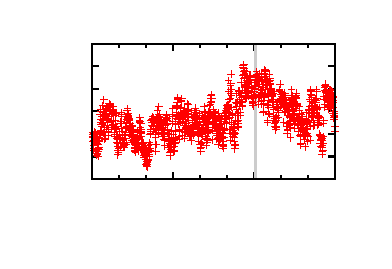
\includegraphics{/home/rik/workspace/ASL_student_project/Repositories/report-fork/Report/images/windminute}}%
    \gplfronttext
  \end{picture}%
\endgroup

\label{fig:wind_speed_minutes}}
\subfloat[][{Wind azimuth $[ \si{\degree} ]$ from \formattime{5}{30}{0} to \formattime{5}{33}{0}  }]{
\input{images/windaziminute.tex}
\label{fig:wind_azi_minutes}}
\caption[Wind observations]{Wind observations. The data is gathered using an anemometer $2.76 \si{\metre}$ above ground in an open field in California, USA. More information and measurement data can be found in Google's open source data collection \cite{www:googleosb,www:googleheliostat}.}
\label{fig:wind_observations}
\end{figure}


In the bottom picture \subref{fig:wind_speed_minutes} one can detect a wind gust at \formattime{5}{32}{0}. The wind velocity suddenly reaches a peak of $10 \si{\metre\per\second}$ after averaging around $5 \si{\metre\per\second}$. 

However, the MAV position control action takes place in a even smaller time interval. For visualization a $3 \si{\second}$ interval has been highlighted with a vertical grey line in figure \ref{fig:wind_observations} \subref{fig:wind_speed_minutes} and \subref{fig:wind_azi_minutes}. 

Within this small time window the wind field can be modeled as a stationary stochastic process. The wind speed vector is characterised by a constant mean and variance.

\begin{align}
\E[\mathbf{w}(t)] &= \mean{\mathbf{w}} \\
\Var[\mathbf{w}(t)] &= \E\left[\left(\mathbf{w}(t)-\mean{\mathbf{w}} \right) \left(\mathbf{w}(t)-\mean{\mathbf{w}} \right)^T \right]  =\mathbf{ \Sigma }
\end{align}

Thus the differential equation governing the wind field is
\begin{align}
\d{\mathbf{w}(t)} &= \mathbf{ \Sigma } \d{\mathbf{W}(t)} \\
\mathbf{w}(0) &= \mean{\mathbf{w}}
\end{align}
where $\mathbf{W}(t)$ is standard Brownian motion.

A more convenient way is to state the dynamics as a discrete-time state space systems.
\begin{align}
\mathbf{w}(k+1) &= \mathbf{w}(k) + \mathbf{Q} \boldsymbol{\varepsilon}(k) \\ 
{\varepsilon}_i (k) &\sim \mathcal{N}(0,1) & \forall i \in \{ x,y,z \}
\label{eq:wind_state_space}
\end{align}


\subsection{Wind Forces}
Wind affects the MAV dynamics in two ways. On one hand it causes pressure on the multirotor surface opposed to the wind field. We call this load area drag $\mathbf{F}_A$. On the other hand the wind field influences the total rotor drag. We name this load drag force $\mathbf{F}_D$.

Schiano and others examined the effects of area drag on a Parrot AR Drone 2.0 (quadrotor) without polystyrene casing \cite{Schiano2014,www:parrot}. This MAV is a little smaller than the AscTec Firefly but the results are qualitatively comparable. They described area drag according to Rayleigh equations.

\begin{align}
\mathbf{F}_A = \frac{1}{2} C_A \rho \norm{\mathbf{w}}_2 \mathbf{w}  \label{eq:area_drag}
\end{align}
with
\begin{align*}
C_A&: & \text{area drag coefficient} \\
\rho&: &\text{air density} \\
\mathbf{w}&: &\text{wind speed}.
\end{align*}

In wind tunnel experiments they measured the forces on the switched off MAV for different angles of attack. They concluded that the drag coefficient is mainly a function of heading towards the wind. The worst case (largest force) equaled to $\psi = 90 \si{\degree}$, when the processor housing is exposed with the long side and thus the largest area towards the wind. 

Following rotor blade theory, the drag force is given as in equation \ref{eq:drag_force}.
\begin{align}
\mathbf{F}_D&= \sum_{i=1}^6 \omega_i \cdot  C_D \cdot _B\mathbf{\mathbf{w}}^\perp
\end{align}

Using the worst case area drag coefficient $C_A = 0.02$ from Schianos experiments and the rotor drag coefficent $C_D = \num{6.84 e-5}$ for the Firefly we simulate the resulting forces. Figure \ref{fig:area_vs_rotor_drag} shows the area and the rotor drag at different wind speeds and a hovering Firefly.    

\begin{figure} 
\centering 
% This file was created by matlab2tikz.
% Minimal pgfplots version: 1.3
%
%The latest updates can be retrieved from
%  http://www.mathworks.com/matlabcentral/fileexchange/22022-matlab2tikz
%where you can also make suggestions and rate matlab2tikz.
%
\definecolor{mycolor1}{rgb}{0.00000,0.44700,0.74100}%
\definecolor{mycolor2}{rgb}{0.85000,0.32500,0.09800}%
%
\begin{tikzpicture}

\begin{axis}[%
width=\figurewidth,
height=0.939692\figureheight,
at={(0\figurewidth,0\figureheight)},
scale only axis,
xmin=0,
xmax=25,
xtick={ 0,  5, 10, 15, 20, 25},
xlabel={Wind velocity $[\si{\metre\per\second}]$},
ymin=0,
ymax=8,
ytick={ 0,  1,  2,  3,  4,  5,  6,  7,  8,  9, 10},
ylabel={Drag force [\si{\newton}]},
legend style={at={(0.5,1.03)},anchor=south,legend columns=2,legend cell align=left,align=left,draw=white!15!black}
]
\addplot [color=mycolor1,solid]
  table[row sep=crcr]{%
0	0\\
0.025025025025025	7.67158549941333e-06\\
0.0500500500500501	3.06863419976533e-05\\
0.0750750750750751	6.90442694947199e-05\\
0.1001001001001	0.000122745367990613\\
0.125125125125125	0.000191789637485333\\
0.15015015015015	0.00027617707797888\\
0.175175175175175	0.000375907689471253\\
0.2002002002002	0.000490981471962453\\
0.225225225225225	0.00062139842545248\\
0.25025025025025	0.000767158549941333\\
0.275275275275275	0.000928261845429013\\
0.3003003003003	0.00110470831191552\\
0.325325325325325	0.00129649794940085\\
0.35035035035035	0.00150363075788501\\
0.375375375375375	0.001726106737368\\
0.4004004004004	0.00196392588784981\\
0.425425425425425	0.00221708820933045\\
0.45045045045045	0.00248559370180992\\
0.475475475475475	0.00276944236528821\\
0.500500500500501	0.00306863419976533\\
0.525525525525526	0.00338316920524128\\
0.550550550550551	0.00371304738171605\\
0.575575575575576	0.00405826872918965\\
0.600600600600601	0.00441883324766208\\
0.625625625625626	0.00479474093713333\\
0.650650650650651	0.00518599179760341\\
0.675675675675676	0.00559258582907231\\
0.700700700700701	0.00601452303154005\\
0.725725725725726	0.00645180340500661\\
0.750750750750751	0.00690442694947199\\
0.775775775775776	0.00737239366493621\\
0.800800800800801	0.00785570355139925\\
0.825825825825826	0.00835435660886111\\
0.850850850850851	0.00886835283732181\\
0.875875875875876	0.00939769223678133\\
0.900900900900901	0.00994237480723967\\
0.925925925925926	0.0105024005486968\\
0.950950950950951	0.0110777694611528\\
0.975975975975976	0.0116684815446077\\
1.001001001001	0.0122745367990613\\
1.02602602602603	0.0128959352245138\\
1.05105105105105	0.0135326768209651\\
1.07607607607608	0.0141847615884152\\
1.1011011011011	0.0148521895268642\\
1.12612612612613	0.015534960636312\\
1.15115115115115	0.0162330749167586\\
1.17617617617618	0.016946532368204\\
1.2012012012012	0.0176753329906483\\
1.22622622622623	0.0184194767840914\\
1.25125125125125	0.0191789637485333\\
1.27627627627628	0.0199537938839741\\
1.3013013013013	0.0207439671904136\\
1.32632632632633	0.021549483667852\\
1.35135135135135	0.0223703433162893\\
1.37637637637638	0.0232065461357253\\
1.4014014014014	0.0240580921261602\\
1.42642642642643	0.0249249812875939\\
1.45145145145145	0.0258072136200264\\
1.47647647647648	0.0267047891234578\\
1.5015015015015	0.027617707797888\\
1.52652652652653	0.028545969643317\\
1.55155155155155	0.0294895746597448\\
1.57657657657658	0.0304485228471715\\
1.6016016016016	0.031422814205597\\
1.62662662662663	0.0324124487350213\\
1.65165165165165	0.0334174264354445\\
1.67667667667668	0.0344377473068664\\
1.7017017017017	0.0354734113492872\\
1.72672672672673	0.0365244185627069\\
1.75175175175175	0.0375907689471253\\
1.77677677677678	0.0386724625025426\\
1.8018018018018	0.0397694992289587\\
1.82682682682683	0.0408818791263736\\
1.85185185185185	0.0420096021947874\\
1.87687687687688	0.0431526684342\\
1.9019019019019	0.0443110778446114\\
1.92692692692693	0.0454848304260216\\
1.95195195195195	0.0466739261784307\\
1.97697697697698	0.0478783651018386\\
2.002002002002	0.0490981471962453\\
2.02702702702703	0.0503332724616509\\
2.05205205205205	0.0515837408980552\\
2.07707707707708	0.0528495525054584\\
2.1021021021021	0.0541307072838604\\
2.12712712712713	0.0554272052332613\\
2.15215215215215	0.056739046353661\\
2.17717717717718	0.0580662306450595\\
2.2022022022022	0.0594087581074568\\
2.22722722722723	0.060766628740853\\
2.25225225225225	0.062139842545248\\
2.27727727727728	0.0635283995206418\\
2.3023023023023	0.0649322996670344\\
2.32732732732733	0.0663515429844259\\
2.35235235235235	0.0677861294728162\\
2.37737737737738	0.0692360591322053\\
2.4024024024024	0.0707013319625932\\
2.42742742742743	0.07218194796398\\
2.45245245245245	0.0736779071363656\\
2.47747747747748	0.07518920947975\\
2.5025025025025	0.0767158549941333\\
2.52752752752753	0.0782578436795154\\
2.55255255255255	0.0798151755358963\\
2.57757757757758	0.081387850563276\\
2.6026026026026	0.0829758687616546\\
2.62762762762763	0.0845792301310319\\
2.65265265265265	0.0861979346714081\\
2.67767767767768	0.0878319823827832\\
2.7027027027027	0.089481373265157\\
2.72772772772773	0.0911461073185297\\
2.75275275275275	0.0928261845429013\\
2.77777777777778	0.0945216049382716\\
2.8028028028028	0.0962323685046408\\
2.82782782782783	0.0979584752420088\\
2.85285285285285	0.0996999251503756\\
2.87787787787788	0.101456718229741\\
2.9029029029029	0.103228854480106\\
2.92792792792793	0.105016333901469\\
2.95295295295295	0.106819156493831\\
2.97797797797798	0.108637322257192\\
3.003003003003	0.110470831191552\\
3.02802802802803	0.112319683296911\\
3.05305305305305	0.114183878573268\\
3.07807807807808	0.116063417020624\\
3.1031031031031	0.117958298638979\\
3.12812812812813	0.119868523428333\\
3.15315315315315	0.121794091388686\\
3.17817817817818	0.123735002520038\\
3.2032032032032	0.125691256822388\\
3.22822822822823	0.127662854295737\\
3.25325325325325	0.129649794940085\\
3.27827827827828	0.131652078755432\\
3.3033033033033	0.133669705741778\\
3.32832832832833	0.135702675899122\\
3.35335335335335	0.137750989227466\\
3.37837837837838	0.139814645726808\\
3.4034034034034	0.141893645397149\\
3.42842842842843	0.143987988238489\\
3.45345345345345	0.146097674250827\\
3.47847847847848	0.148222703434165\\
3.5035035035035	0.150363075788501\\
3.52852852852853	0.152518791313836\\
3.55355355355355	0.15468985001017\\
3.57857857857858	0.156876251877503\\
3.6036036036036	0.159077996915835\\
3.62862862862863	0.161295085125165\\
3.65365365365365	0.163527516505494\\
3.67867867867868	0.165775291056823\\
3.7037037037037	0.16803840877915\\
3.72872872872873	0.170316869672475\\
3.75375375375375	0.1726106737368\\
3.77877877877878	0.174919820972123\\
3.8038038038038	0.177244311378446\\
3.82882882882883	0.179584144955767\\
3.85385385385385	0.181939321704086\\
3.87887887887888	0.184309841623405\\
3.9039039039039	0.186695704713723\\
3.92892892892893	0.189096910975039\\
3.95395395395395	0.191513460407354\\
3.97897897897898	0.193945353010668\\
4.004004004004	0.196392588784981\\
4.02902902902903	0.198855167730293\\
4.05405405405405	0.201333089846603\\
4.07907907907908	0.203826355133913\\
4.1041041041041	0.206334963592221\\
4.12912912912913	0.208858915221528\\
4.15415415415415	0.211398210021834\\
4.17917917917918	0.213952847993138\\
4.2042042042042	0.216522829135442\\
4.22922922922923	0.219108153448744\\
4.25425425425425	0.221708820933045\\
4.27927927927928	0.224324831588345\\
4.3043043043043	0.226956185414644\\
4.32932932932933	0.229602882411941\\
4.35435435435435	0.232264922580238\\
4.37937937937938	0.234942305919533\\
4.4044044044044	0.237635032429827\\
4.42942942942943	0.24034310211112\\
4.45445445445445	0.243066514963412\\
4.47947947947948	0.245805270986702\\
4.5045045045045	0.248559370180992\\
4.52952952952953	0.25132881254628\\
4.55455455455455	0.254113598082567\\
4.57957957957958	0.256913726789853\\
4.6046046046046	0.259729198668138\\
4.62962962962963	0.262560013717421\\
4.65465465465465	0.265406171937703\\
4.67967967967968	0.268267673328985\\
4.7047047047047	0.271144517891265\\
4.72972972972973	0.274036705624543\\
4.75475475475475	0.276944236528821\\
4.77977977977978	0.279867110604098\\
4.8048048048048	0.282805327850373\\
4.82982982982983	0.285758888267647\\
4.85485485485485	0.28872779185592\\
4.87987987987988	0.291712038615192\\
4.9049049049049	0.294711628545462\\
4.92992992992993	0.297726561646732\\
4.95495495495495	0.300756837919\\
4.97997997997998	0.303802457362267\\
5.00500500500501	0.306863419976533\\
5.03003003003003	0.309939725761798\\
5.05505505505506	0.313031374718061\\
5.08008008008008	0.316138366845324\\
5.10510510510511	0.319260702143585\\
5.13013013013013	0.322398380612845\\
5.15515515515516	0.325551402253104\\
5.18018018018018	0.328719767064362\\
5.20520520520521	0.331903475046618\\
5.23023023023023	0.335102526199874\\
5.25525525525526	0.338316920524128\\
5.28028028028028	0.341546658019381\\
5.30530530530531	0.344791738685633\\
5.33033033033033	0.348052162522883\\
5.35535535535536	0.351327929531133\\
5.38038038038038	0.354619039710381\\
5.40540540540541	0.357925493060628\\
5.43043043043043	0.361247289581874\\
5.45545545545546	0.364584429274119\\
5.48048048048048	0.367936912137363\\
5.50550550550551	0.371304738171605\\
5.53053053053053	0.374687907376846\\
5.55555555555556	0.378086419753086\\
5.58058058058058	0.381500275300325\\
5.60560560560561	0.384929474018563\\
5.63063063063063	0.3883740159078\\
5.65565565565566	0.391833900968035\\
5.68068068068068	0.395309129199269\\
5.70570570570571	0.398799700601502\\
5.73073073073073	0.402305615174734\\
5.75575575575576	0.405826872918965\\
5.78078078078078	0.409363473834195\\
5.80580580580581	0.412915417920423\\
5.83083083083083	0.41648270517765\\
5.85585585585586	0.420065335605876\\
5.88088088088088	0.423663309205101\\
5.90590590590591	0.427276625975325\\
5.93093093093093	0.430905285916547\\
5.95595595595596	0.434549289028768\\
5.98098098098098	0.438208635311989\\
6.00600600600601	0.441883324766208\\
6.03103103103103	0.445573357391425\\
6.05605605605606	0.449278733187642\\
6.08108108108108	0.452999452154858\\
6.10610610610611	0.456735514293072\\
6.13113113113113	0.460486919602285\\
6.15615615615616	0.464253668082497\\
6.18118118118118	0.468035759733708\\
6.20620620620621	0.471833194555917\\
6.23123123123123	0.475645972549126\\
6.25625625625626	0.479474093713333\\
6.28128128128128	0.483317558048539\\
6.30630630630631	0.487176365554744\\
6.33133133133133	0.491050516231948\\
6.35635635635636	0.49494001008015\\
6.38138138138138	0.498844847099352\\
6.40640640640641	0.502765027289552\\
6.43143143143143	0.506700550650751\\
6.45645645645646	0.510651417182949\\
6.48148148148148	0.514617626886145\\
6.50650650650651	0.518599179760341\\
6.53153153153153	0.522596075805535\\
6.55655655655656	0.526608315021728\\
6.58158158158158	0.530635897408921\\
6.60660660660661	0.534678822967111\\
6.63163163163163	0.538737091696301\\
6.65665665665666	0.542810703596489\\
6.68168168168168	0.546899658667677\\
6.70670670670671	0.551003956909863\\
6.73173173173173	0.555123598323048\\
6.75675675675676	0.559258582907232\\
6.78178178178178	0.563408910662414\\
6.80680680680681	0.567574581588596\\
6.83183183183183	0.571755595685776\\
6.85685685685686	0.575951952953955\\
6.88188188188188	0.580163653393133\\
6.90690690690691	0.58439069700331\\
6.93193193193193	0.588633083784485\\
6.95695695695696	0.59289081373666\\
6.98198198198198	0.597163886859833\\
7.00700700700701	0.601452303154005\\
7.03203203203203	0.605756062619176\\
7.05705705705706	0.610075165255346\\
7.08208208208208	0.614409611062514\\
7.10710710710711	0.618759400040681\\
7.13213213213213	0.623124532189848\\
7.15715715715716	0.627505007510013\\
7.18218218218218	0.631900826001176\\
7.20720720720721	0.636311987663339\\
7.23223223223223	0.640738492496501\\
7.25725725725726	0.645180340500661\\
7.28228228228228	0.64963753167582\\
7.30730730730731	0.654110066021978\\
7.33233233233233	0.658597943539135\\
7.35735735735736	0.66310116422729\\
7.38238238238238	0.667619728086445\\
7.40740740740741	0.672153635116598\\
7.43243243243243	0.67670288531775\\
7.45745745745746	0.681267478689901\\
7.48248248248248	0.685847415233051\\
7.50750750750751	0.690442694947199\\
7.53253253253253	0.695053317832347\\
7.55755755755756	0.699679283888493\\
7.58258258258258	0.704320593115638\\
7.60760760760761	0.708977245513782\\
7.63263263263263	0.713649241082925\\
7.65765765765766	0.718336579823066\\
7.68268268268268	0.723039261734207\\
7.70770770770771	0.727757286816346\\
7.73273273273273	0.732490655069484\\
7.75775775775776	0.737239366493621\\
7.78278278278278	0.742003421088756\\
7.80780780780781	0.746782818854891\\
7.83283283283283	0.751577559792024\\
7.85785785785786	0.756387643900156\\
7.88288288288288	0.761213071179287\\
7.90790790790791	0.766053841629417\\
7.93293293293293	0.770909955250546\\
7.95795795795796	0.775781412042673\\
7.98298298298298	0.7806682120058\\
8.00800800800801	0.785570355139925\\
8.03303303303303	0.790487841445049\\
8.05805805805806	0.795420670921172\\
8.08308308308308	0.800368843568293\\
8.10810810810811	0.805332359386414\\
8.13313313313313	0.810311218375533\\
8.15815815815816	0.815305420535651\\
8.18318318318318	0.820314965866768\\
8.20820820820821	0.825339854368884\\
8.23323323323323	0.830380086041998\\
8.25825825825826	0.835435660886112\\
8.28328328328328	0.840506578901224\\
8.30830830830831	0.845592840087335\\
8.33333333333333	0.850694444444445\\
8.35835835835836	0.855811391972553\\
8.38338338338338	0.860943682671661\\
8.40840840840841	0.866091316541767\\
8.43343343343343	0.871254293582872\\
8.45845845845846	0.876432613794976\\
8.48348348348348	0.881626277178079\\
8.50850850850851	0.886835283732181\\
8.53353353353353	0.892059633457281\\
8.55855855855856	0.89729932635338\\
8.58358358358358	0.902554362420479\\
8.60860860860861	0.907824741658576\\
8.63363363363363	0.913110464067671\\
8.65865865865866	0.918411529647766\\
8.68368368368368	0.923727938398859\\
8.70870870870871	0.929059690320952\\
8.73373373373373	0.934406785414043\\
8.75875875875876	0.939769223678133\\
8.78378378378378	0.945147005113221\\
8.80880880880881	0.950540129719309\\
8.83383383383383	0.955948597496395\\
8.85885885885886	0.961372408444481\\
8.88388388388388	0.966811562563565\\
8.90890890890891	0.972266059853648\\
8.93393393393393	0.977735900314729\\
8.95895895895896	0.98322108394681\\
8.98398398398398	0.988721610749889\\
9.00900900900901	0.994237480723967\\
9.03403403403403	0.999768693869044\\
9.05905905905906	1.00531525018512\\
9.08408408408408	1.01087714967219\\
9.10910910910911	1.01645439233027\\
9.13413413413413	1.02204697815934\\
9.15915915915916	1.02765490715941\\
9.18418418418418	1.03327817933048\\
9.20920920920921	1.03891679467255\\
9.23423423423423	1.04457075318562\\
9.25925925925926	1.05024005486968\\
9.28428428428428	1.05592469972475\\
9.30930930930931	1.06162468775081\\
9.33433433433433	1.06734001894788\\
9.35935935935936	1.07307069331594\\
9.38438438438438	1.078816710855\\
9.40940940940941	1.08457807156506\\
9.43443443443443	1.09035477544612\\
9.45945945945946	1.09614682249817\\
9.48448448448448	1.10195421272123\\
9.50950950950951	1.10777694611528\\
9.53453453453453	1.11361502268034\\
9.55955955955956	1.11946844241639\\
9.58458458458458	1.12533720532344\\
9.60960960960961	1.13122131140149\\
9.63463463463463	1.13712076065054\\
9.65965965965966	1.14303555307059\\
9.68468468468468	1.14896568866163\\
9.70970970970971	1.15491116742368\\
9.73473473473473	1.16087198935672\\
9.75975975975976	1.16684815446077\\
9.78478478478478	1.17283966273581\\
9.80980980980981	1.17884651418185\\
9.83483483483483	1.18486870879889\\
9.85985985985986	1.19090624658693\\
9.88488488488488	1.19695912754596\\
9.90990990990991	1.203027351676\\
9.93493493493493	1.20911091897704\\
9.95995995995996	1.21520982944907\\
9.98498498498498	1.2213240830921\\
10.01001001001	1.22745367990613\\
10.035035035035	1.23359861989116\\
10.0600600600601	1.23975890304719\\
10.0850850850851	1.24593452937422\\
10.1101101101101	1.25212549887225\\
10.1351351351351	1.25833181154127\\
10.1601601601602	1.2645534673813\\
10.1851851851852	1.27079046639232\\
10.2102102102102	1.27704280857434\\
10.2352352352352	1.28331049392736\\
10.2602602602603	1.28959352245138\\
10.2852852852853	1.2958918941464\\
10.3103103103103	1.30220560901242\\
10.3353353353353	1.30853466704943\\
10.3603603603604	1.31487906825745\\
10.3853853853854	1.32123881263646\\
10.4104104104104	1.32761390018647\\
10.4354354354354	1.33400433090748\\
10.4604604604605	1.34041010479949\\
10.4854854854855	1.3468312218625\\
10.5105105105105	1.35326768209651\\
10.5355355355355	1.35971948550152\\
10.5605605605606	1.36618663207752\\
10.5855855855856	1.37266912182453\\
10.6106106106106	1.37916695474253\\
10.6356356356356	1.38568013083153\\
10.6606606606607	1.39220865009153\\
10.6856856856857	1.39875251252253\\
10.7107107107107	1.40531171812453\\
10.7357357357357	1.41188626689753\\
10.7607607607608	1.41847615884152\\
10.7857857857858	1.42508139395652\\
10.8108108108108	1.43170197224251\\
10.8358358358358	1.43833789369951\\
10.8608608608609	1.4449891583275\\
10.8858858858859	1.45165576612649\\
10.9109109109109	1.45833771709648\\
10.9359359359359	1.46503501123746\\
10.960960960961	1.47174764854945\\
10.985985985986	1.47847562903244\\
11.011011011011	1.48521895268642\\
11.036036036036	1.4919776195114\\
11.0610610610611	1.49875162950739\\
11.0860860860861	1.50554098267437\\
11.1111111111111	1.51234567901235\\
11.1361361361361	1.51916571852132\\
11.1611611611612	1.5260011012013\\
11.1861861861862	1.53285182705228\\
11.2112112112112	1.53971789607425\\
11.2362362362362	1.54659930826723\\
11.2612612612613	1.5534960636312\\
11.2862862862863	1.56040816216617\\
11.3113113113113	1.56733560387214\\
11.3363363363363	1.57427838874911\\
11.3613613613614	1.58123651679708\\
11.3863863863864	1.58820998801604\\
11.4114114114114	1.59519880240601\\
11.4364364364364	1.60220295996697\\
11.4614614614615	1.60922246069894\\
11.4864864864865	1.6162573046019\\
11.5115115115115	1.62330749167586\\
11.5365365365365	1.63037302192082\\
11.5615615615616	1.63745389533678\\
11.5865865865866	1.64455011192374\\
11.6116116116116	1.65166167168169\\
11.6366366366366	1.65878857461065\\
11.6616616616617	1.6659308207106\\
11.6866866866867	1.67308840998155\\
11.7117117117117	1.6802613424235\\
11.7367367367367	1.68744961803645\\
11.7617617617618	1.6946532368204\\
11.7867867867868	1.70187219877535\\
11.8118118118118	1.7091065039013\\
11.8368368368368	1.71635615219824\\
11.8618618618619	1.72362114366619\\
11.8868868868869	1.73090147830513\\
11.9119119119119	1.73819715611507\\
11.9369369369369	1.74550817709601\\
11.961961961962	1.75283454124795\\
11.986986986987	1.76017624857089\\
12.012012012012	1.76753329906483\\
12.037037037037	1.77490569272977\\
12.0620620620621	1.7822934295657\\
12.0870870870871	1.78969650957264\\
12.1121121121121	1.79711493275057\\
12.1371371371371	1.8045486990995\\
12.1621621621622	1.81199780861943\\
12.1871871871872	1.81946226131036\\
12.2122122122122	1.82694205717229\\
12.2372372372372	1.83443719620521\\
12.2622622622623	1.84194767840914\\
12.2872872872873	1.84947350378406\\
12.3123123123123	1.85701467232999\\
12.3373373373373	1.86457118404691\\
12.3623623623624	1.87214303893483\\
12.3873873873874	1.87973023699375\\
12.4124124124124	1.88733277822367\\
12.4374374374374	1.89495066262459\\
12.4624624624625	1.9025838901965\\
12.4874874874875	1.91023246093942\\
12.5125125125125	1.91789637485333\\
12.5375375375375	1.92557563193824\\
12.5625625625626	1.93327023219416\\
12.5875875875876	1.94098017562107\\
12.6126126126126	1.94870546221898\\
12.6376376376376	1.95644609198788\\
12.6626626626627	1.96420206492779\\
12.6876876876877	1.9719733810387\\
12.7127127127127	1.9797600403206\\
12.7377377377377	1.9875620427735\\
12.7627627627628	1.99537938839741\\
12.7877877877878	2.00321207719231\\
12.8128128128128	2.01106010915821\\
12.8378378378378	2.01892348429511\\
12.8628628628629	2.026802202603\\
12.8878878878879	2.0346962640819\\
12.9129129129129	2.0426056687318\\
12.9379379379379	2.05053041655269\\
12.962962962963	2.05847050754458\\
12.987987987988	2.06642594170747\\
13.013013013013	2.07439671904136\\
13.038038038038	2.08238283954625\\
13.0630630630631	2.09038430322214\\
13.0880880880881	2.09840111006903\\
13.1131131131131	2.10643326008691\\
13.1381381381381	2.1144807532758\\
13.1631631631632	2.12254358963568\\
13.1881881881882	2.13062176916656\\
13.2132132132132	2.13871529186845\\
13.2382382382382	2.14682415774133\\
13.2632632632633	2.1549483667852\\
13.2882882882883	2.16308791900008\\
13.3133133133133	2.17124281438596\\
13.3383383383383	2.17941305294283\\
13.3633633633634	2.18759863467071\\
13.3883883883884	2.19579955956958\\
13.4134134134134	2.20401582763945\\
13.4384384384384	2.21224743888032\\
13.4634634634635	2.22049439329219\\
13.4884884884885	2.22875669087506\\
13.5135135135135	2.23703433162893\\
13.5385385385385	2.24532731555379\\
13.5635635635636	2.25363564264966\\
13.5885885885886	2.26195931291652\\
13.6136136136136	2.27029832635438\\
13.6386386386386	2.27865268296324\\
13.6636636636637	2.2870223827431\\
13.6886886886887	2.29540742569396\\
13.7137137137137	2.30380781181582\\
13.7387387387387	2.31222354110868\\
13.7637637637638	2.32065461357253\\
13.7887887887888	2.32910102920739\\
13.8138138138138	2.33756278801324\\
13.8388388388388	2.34603988999009\\
13.8638638638639	2.35453233513794\\
13.8888888888889	2.36304012345679\\
13.9139139139139	2.37156325494664\\
13.9389389389389	2.38010172960749\\
13.963963963964	2.38865554743933\\
13.988988988989	2.39722470844218\\
14.014014014014	2.40580921261602\\
14.039039039039	2.41440905996086\\
14.0640640640641	2.4230242504767\\
14.0890890890891	2.43165478416354\\
14.1141141141141	2.44030066102138\\
14.1391391391391	2.44896188105022\\
14.1641641641642	2.45763844425006\\
14.1891891891892	2.46633035062089\\
14.2142142142142	2.47503760016273\\
14.2392392392392	2.48376019287556\\
14.2642642642643	2.49249812875939\\
14.2892892892893	2.50125140781422\\
14.3143143143143	2.51002003004005\\
14.3393393393393	2.51880399543688\\
14.3643643643644	2.52760330400471\\
14.3893893893894	2.53641795574353\\
14.4144144144144	2.54524795065336\\
14.4394394394394	2.55409328873418\\
14.4644644644645	2.562953969986\\
14.4894894894895	2.57182999440882\\
14.5145145145145	2.58072136200264\\
14.5395395395395	2.58962807276746\\
14.5645645645646	2.59855012670328\\
14.5895895895896	2.6074875238101\\
14.6146146146146	2.61644026408791\\
14.6396396396396	2.62540834753673\\
14.6646646646647	2.63439177415654\\
14.6896896896897	2.64339054394735\\
14.7147147147147	2.65240465690916\\
14.7397397397397	2.66143411304197\\
14.7647647647648	2.67047891234578\\
14.7897897897898	2.67953905482059\\
14.8148148148148	2.68861454046639\\
14.8398398398398	2.6977053692832\\
14.8648648648649	2.706811541271\\
14.8898898898899	2.7159330564298\\
14.9149149149149	2.7250699147596\\
14.9399399399399	2.7342221162604\\
14.964964964965	2.7433896609322\\
14.98998998999	2.752572548775\\
15.015015015015	2.7617707797888\\
15.04004004004	2.77098435397359\\
15.0650650650651	2.78021327132939\\
15.0900900900901	2.78945753185618\\
15.1151151151151	2.79871713555397\\
15.1401401401401	2.80799208242276\\
15.1651651651652	2.81728237246255\\
15.1901901901902	2.82658800567334\\
15.2152152152152	2.83590898205513\\
15.2402402402402	2.84524530160791\\
15.2652652652653	2.8545969643317\\
15.2902902902903	2.86396397022648\\
15.3153153153153	2.87334631929227\\
15.3403403403403	2.88274401152905\\
15.3653653653654	2.89215704693683\\
15.3903903903904	2.90158542551561\\
15.4154154154154	2.91102914726538\\
15.4404404404404	2.92048821218616\\
15.4654654654655	2.92996262027794\\
15.4904904904905	2.93945237154071\\
15.5155155155155	2.94895746597448\\
15.5405405405405	2.95847790357925\\
15.5655655655656	2.96801368435503\\
15.5905905905906	2.9775648083018\\
15.6156156156156	2.98713127541956\\
15.6406406406406	2.99671308570833\\
15.6656656656657	3.0063102391681\\
15.6906906906907	3.01592273579886\\
15.7157157157157	3.02555057560063\\
15.7407407407407	3.03519375857339\\
15.7657657657658	3.04485228471715\\
15.7907907907908	3.05452615403191\\
15.8158158158158	3.06421536651767\\
15.8408408408408	3.07391992217443\\
15.8658658658659	3.08363982100218\\
15.8908908908909	3.09337506300094\\
15.9159159159159	3.10312564817069\\
15.9409409409409	3.11289157651145\\
15.965965965966	3.1226728480232\\
15.990990990991	3.13246946270595\\
16.016016016016	3.1422814205597\\
16.041041041041	3.15210872158445\\
16.0660660660661	3.1619513657802\\
16.0910910910911	3.17180935314694\\
16.1161161161161	3.18168268368469\\
16.1411411411411	3.19157135739343\\
16.1661661661662	3.20147537427317\\
16.1911911911912	3.21139473432391\\
16.2162162162162	3.22132943754565\\
16.2412412412412	3.23127948393839\\
16.2662662662663	3.24124487350213\\
16.2912912912913	3.25122560623687\\
16.3163163163163	3.2612216821426\\
16.3413413413413	3.27123310121934\\
16.3663663663664	3.28125986346707\\
16.3913913913914	3.2913019688858\\
16.4164164164164	3.30135941747553\\
16.4414414414414	3.31143220923626\\
16.4664664664665	3.32152034416799\\
16.4914914914915	3.33162382227072\\
16.5165165165165	3.34174264354445\\
16.5415415415415	3.35187680798917\\
16.5665665665666	3.36202631560489\\
16.5915915915916	3.37219116639162\\
16.6166166166166	3.38237136034934\\
16.6416416416416	3.39256689747806\\
16.6666666666667	3.40277777777778\\
16.6916916916917	3.4130040012485\\
16.7167167167167	3.42324556789021\\
16.7417417417417	3.43350247770293\\
16.7667667667668	3.44377473068664\\
16.7917917917918	3.45406232684136\\
16.8168168168168	3.46436526616707\\
16.8418418418418	3.47468354866378\\
16.8668668668669	3.48501717433149\\
16.8918918918919	3.4953661431702\\
16.9169169169169	3.50573045517991\\
16.9419419419419	3.51611011036061\\
16.966966966967	3.52650510871232\\
16.991991991992	3.53691545023502\\
17.017017017017	3.54734113492872\\
17.042042042042	3.55778216279342\\
17.0670670670671	3.56823853382912\\
17.0920920920921	3.57871024803582\\
17.1171171171171	3.58919730541352\\
17.1421421421421	3.59969970596222\\
17.1671671671672	3.61021744968191\\
17.1921921921922	3.62075053657261\\
17.2172172172172	3.6312989666343\\
17.2422422422422	3.64186273986699\\
17.2672672672673	3.65244185627069\\
17.2922922922923	3.66303631584537\\
17.3173173173173	3.67364611859106\\
17.3423423423423	3.68427126450775\\
17.3673673673674	3.69491175359544\\
17.3923923923924	3.70556758585412\\
17.4174174174174	3.71623876128381\\
17.4424424424424	3.72692527988449\\
17.4674674674675	3.73762714165617\\
17.4924924924925	3.74834434659885\\
17.5175175175175	3.75907689471253\\
17.5425425425425	3.76982478599721\\
17.5675675675676	3.78058802045289\\
17.5925925925926	3.79136659807956\\
17.6176176176176	3.80216051887724\\
17.6426426426426	3.81296978284591\\
17.6676676676677	3.82379438998558\\
17.6926926926927	3.83463434029625\\
17.7177177177177	3.84548963377792\\
17.7427427427427	3.85636027043059\\
17.7677677677678	3.86724625025426\\
17.7927927927928	3.87814757324892\\
17.8178178178178	3.88906423941459\\
17.8428428428428	3.89999624875125\\
17.8678678678679	3.91094360125892\\
17.8928928928929	3.92190629693758\\
17.9179179179179	3.93288433578724\\
17.9429429429429	3.9438777178079\\
17.967967967968	3.95488644299956\\
17.992992992993	3.96591051136221\\
18.018018018018	3.97694992289587\\
18.043043043043	3.98800467760052\\
18.0680680680681	3.99907477547618\\
18.0930930930931	4.01016021652283\\
18.1181181181181	4.02126100074048\\
18.1431431431431	4.03237712812913\\
18.1681681681682	4.04350859868878\\
18.1931931931932	4.05465541241943\\
18.2182182182182	4.06581756932107\\
18.2432432432432	4.07699506939372\\
18.2682682682683	4.08818791263736\\
18.2932932932933	4.099396099052\\
18.3183183183183	4.11061962863765\\
18.3433433433433	4.12185850139429\\
18.3683683683684	4.13311271732193\\
18.3933933933934	4.14438227642056\\
18.4184184184184	4.1556671786902\\
18.4434434434434	4.16696742413084\\
18.4684684684685	4.17828301274247\\
18.4934934934935	4.1896139445251\\
18.5185185185185	4.20096021947874\\
18.5435435435435	4.21232183760337\\
18.5685685685686	4.223698798899\\
18.5935935935936	4.23509110336563\\
18.6186186186186	4.24649875100326\\
18.6436436436436	4.25792174181188\\
18.6686686686687	4.26936007579151\\
18.6936936936937	4.28081375294213\\
18.7187187187187	4.29228277326375\\
18.7437437437437	4.30376713675638\\
18.7687687687688	4.31526684342\\
18.7937937937938	4.32678189325462\\
18.8188188188188	4.33831228626023\\
18.8438438438438	4.34985802243685\\
18.8688688688689	4.36141910178447\\
18.8938938938939	4.37299552430308\\
18.9189189189189	4.3845872899927\\
18.9439439439439	4.39619439885331\\
18.968968968969	4.40781685088492\\
18.993993993994	4.41945464608753\\
19.019019019019	4.43110778446114\\
19.044044044044	4.44277626600574\\
19.0690690690691	4.45446009072135\\
19.0940940940941	4.46615925860796\\
19.1191191191191	4.47787376966556\\
19.1441441441441	4.48960362389416\\
19.1691691691692	4.50134882129377\\
19.1941941941942	4.51310936186437\\
19.2192192192192	4.52488524560597\\
19.2442442442442	4.53667647251856\\
19.2692692692693	4.54848304260216\\
19.2942942942943	4.56030495585676\\
19.3193193193193	4.57214221228235\\
19.3443443443443	4.58399481187895\\
19.3693693693694	4.59586275464654\\
19.3943943943944	4.60774604058513\\
19.4194194194194	4.61964466969472\\
19.4444444444444	4.63155864197531\\
19.4694694694695	4.6434879574269\\
19.4944944944945	4.65543261604948\\
19.5195195195195	4.66739261784307\\
19.5445445445445	4.67936796280765\\
19.5695695695696	4.69135865094324\\
19.5945945945946	4.70336468224982\\
19.6196196196196	4.7153860567274\\
19.6446446446446	4.72742277437598\\
19.6696696696697	4.73947483519556\\
19.6946946946947	4.75154223918613\\
19.7197197197197	4.76362498634771\\
19.7447447447447	4.77572307668028\\
19.7697697697698	4.78783651018386\\
19.7947947947948	4.79996528685843\\
19.8198198198198	4.812109406704\\
19.8448448448448	4.82426886972057\\
19.8698698698699	4.83644367590814\\
19.8948948948949	4.84863382526671\\
19.9199199199199	4.86083931779627\\
19.9449449449449	4.87306015349684\\
19.96996996997	4.88529633236841\\
19.994994994995	4.89754785441097\\
20.02002002002	4.90981471962453\\
20.045045045045	4.92209692800909\\
20.0700700700701	4.93439447956465\\
20.0950950950951	4.94670737429121\\
20.1201201201201	4.95903561218877\\
20.1451451451451	4.97137919325732\\
20.1701701701702	4.98373811749688\\
20.1951951951952	4.99611238490743\\
20.2202202202202	5.00850199548898\\
20.2452452452452	5.02090694924153\\
20.2702702702703	5.03332724616508\\
20.2952952952953	5.04576288625963\\
20.3203203203203	5.05821386952518\\
20.3453453453453	5.07068019596173\\
20.3703703703704	5.08316186556927\\
20.3953953953954	5.09565887834782\\
20.4204204204204	5.10817123429736\\
20.4454454454454	5.1206989334179\\
20.4704704704705	5.13324197570944\\
20.4954954954955	5.14580036117198\\
20.5205205205205	5.15837408980552\\
20.5455455455455	5.17096316161006\\
20.5705705705706	5.18356757658559\\
20.5955955955956	5.19618733473213\\
20.6206206206206	5.20882243604966\\
20.6456456456456	5.2214728805382\\
20.6706706706707	5.23413866819773\\
20.6956956956957	5.24681979902826\\
20.7207207207207	5.25951627302979\\
20.7457457457457	5.27222809020232\\
20.7707707707708	5.28495525054584\\
20.7957957957958	5.29769775406037\\
20.8208208208208	5.31045560074589\\
20.8458458458458	5.32322879060241\\
20.8708708708709	5.33601732362994\\
20.8958958958959	5.34882119982846\\
20.9209209209209	5.36164041919798\\
20.9459459459459	5.3744749817385\\
20.970970970971	5.38732488745001\\
20.995995995996	5.40019013633253\\
21.021021021021	5.41307072838604\\
21.046046046046	5.42596666361056\\
21.0710710710711	5.43887794200607\\
21.0960960960961	5.45180456357258\\
21.1211211211211	5.46474652831009\\
21.1461461461461	5.4777038362186\\
21.1711711711712	5.49067648729811\\
21.1961961961962	5.50366448154862\\
21.2212212212212	5.51666781897012\\
21.2462462462462	5.52968649956263\\
21.2712712712713	5.54272052332613\\
21.2962962962963	5.55576989026063\\
21.3213213213213	5.56883460036613\\
21.3463463463463	5.58191465364263\\
21.3713713713714	5.59501005009013\\
21.3963963963964	5.60812078970863\\
21.4214214214214	5.62124687249812\\
21.4464464464464	5.63438829845862\\
21.4714714714715	5.64754506759011\\
21.4964964964965	5.66071717989261\\
21.5215215215215	5.6739046353661\\
21.5465465465465	5.68710743401059\\
21.5715715715716	5.70032557582608\\
21.5965965965966	5.71355906081256\\
21.6216216216216	5.72680788897005\\
21.6466466466466	5.74007206029854\\
21.6716716716717	5.75335157479802\\
21.6966966966967	5.76664643246851\\
21.7217217217217	5.77995663330999\\
21.7467467467467	5.79328217732247\\
21.7717717717718	5.80662306450595\\
21.7967967967968	5.81997929486043\\
21.8218218218218	5.8333508683859\\
21.8468468468468	5.84673778508238\\
21.8718718718719	5.86014004494985\\
21.8968968968969	5.87355764798833\\
21.9219219219219	5.8869905941978\\
21.9469469469469	5.90043888357827\\
21.971971971972	5.91390251612974\\
21.996996996997	5.92738149185221\\
22.022022022022	5.94087581074568\\
22.047047047047	5.95438547281015\\
22.0720720720721	5.96791047804561\\
22.0970970970971	5.98145082645208\\
22.1221221221221	5.99500651802954\\
22.1471471471471	6.008577552778\\
22.1721721721722	6.02216393069746\\
22.1971971971972	6.03576565178792\\
22.2222222222222	6.04938271604938\\
22.2472472472472	6.06301512348184\\
22.2722722722723	6.0766628740853\\
22.2972972972973	6.09032596785975\\
22.3223223223223	6.10400440480521\\
22.3473473473473	6.11769818492166\\
22.3723723723724	6.13140730820911\\
22.3973973973974	6.14513177466756\\
22.4224224224224	6.15887158429701\\
22.4474474474474	6.17262673709746\\
22.4724724724725	6.1863972330689\\
22.4974974974975	6.20018307221135\\
22.5225225225225	6.21398425452479\\
22.5475475475475	6.22780078000924\\
22.5725725725726	6.24163264866468\\
22.5975975975976	6.25547986049112\\
22.6226226226226	6.26934241548856\\
22.6476476476476	6.283220313657\\
22.6726726726727	6.29711355499644\\
22.6976976976977	6.31102213950687\\
22.7227227227227	6.32494606718831\\
22.7477477477477	6.33888533804074\\
22.7727727727728	6.35283995206418\\
22.7977977977978	6.36680990925861\\
22.8228228228228	6.38079520962404\\
22.8478478478478	6.39479585316047\\
22.8728728728729	6.4088118398679\\
22.8978978978979	6.42284316974632\\
22.9229229229229	6.43688984279575\\
22.9479479479479	6.45095185901617\\
22.972972972973	6.4650292184076\\
22.997997997998	6.47912192097002\\
23.023023023023	6.49322996670344\\
23.048048048048	6.50735335560786\\
23.0730730730731	6.52149208768328\\
23.0980980980981	6.5356461629297\\
23.1231231231231	6.54981558134711\\
23.1481481481481	6.56400034293553\\
23.1731731731732	6.57820044769494\\
23.1981981981982	6.59241589562536\\
23.2232232232232	6.60664668672677\\
23.2482482482482	6.62089282099918\\
23.2732732732733	6.63515429844259\\
23.2982982982983	6.649431119057\\
23.3233233233233	6.6637232828424\\
23.3483483483483	6.67803078979881\\
23.3733733733734	6.69235363992621\\
23.3983983983984	6.70669183322462\\
23.4234234234234	6.72104536969402\\
23.4484484484484	6.73541424933442\\
23.4734734734735	6.74979847214582\\
23.4984984984985	6.76419803812822\\
23.5235235235235	6.77861294728162\\
23.5485485485485	6.79304319960601\\
23.5735735735736	6.80748879510141\\
23.5985985985986	6.8219497337678\\
23.6236236236236	6.83642601560519\\
23.6486486486486	6.85091764061359\\
23.6736736736737	6.86542460879298\\
23.6986986986987	6.87994692014337\\
23.7237237237237	6.89448457466475\\
23.7487487487487	6.90903757235714\\
23.7737737737738	6.92360591322053\\
23.7987987987988	6.93818959725491\\
23.8238238238238	6.95278862446029\\
23.8488488488488	6.96740299483668\\
23.8738738738739	6.98203270838406\\
23.8988988988989	6.99667776510244\\
23.9239239239239	7.01133816499182\\
23.9489489489489	7.0260139080522\\
23.973973973974	7.04070499428357\\
23.998998998999	7.05541142368595\\
24.024024024024	7.07013319625932\\
24.049049049049	7.0848703120037\\
24.0740740740741	7.09962277091907\\
24.0990990990991	7.11439057300544\\
24.1241241241241	7.12917371826281\\
24.1491491491491	7.14397220669118\\
24.1741741741742	7.15878603829054\\
24.1991991991992	7.17361521306091\\
24.2242242242242	7.18845973100227\\
24.2492492492492	7.20331959211464\\
24.2742742742743	7.218194796398\\
24.2992992992993	7.23308534385236\\
24.3243243243243	7.24799123447772\\
24.3493493493493	7.26291246827408\\
24.3743743743744	7.27784904524144\\
24.3993993993994	7.29280096537979\\
24.4244244244244	7.30776822868915\\
24.4494494494494	7.3227508351695\\
24.4744744744745	7.33774878482086\\
24.4994994994995	7.35276207764321\\
24.5245245245245	7.36779071363656\\
24.5495495495495	7.38283469280091\\
24.5745745745746	7.39789401513626\\
24.5995995995996	7.4129686806426\\
24.6246246246246	7.42805868931995\\
24.6496496496496	7.44316404116829\\
24.6746746746747	7.45828473618764\\
24.6996996996997	7.47342077437798\\
24.7247247247247	7.48857215573932\\
24.7497497497497	7.50373888027166\\
24.7747747747748	7.518920947975\\
24.7997997997998	7.53411835884934\\
24.8248248248248	7.54933111289468\\
24.8498498498498	7.56455921011101\\
24.8748748748749	7.57980265049835\\
24.8998998998999	7.59506143405668\\
24.9249249249249	7.61033556078601\\
24.9499499499499	7.62562503068634\\
24.974974974975	7.64092984375767\\
25	7.65625\\
};
\addlegendentry{Area};

\addplot [color=mycolor2,solid]
  table[row sep=crcr]{%
0	0\\
0.025025025025025	0.0070632445788012\\
0.0500500500500501	0.0141264891576024\\
0.0750750750750751	0.0211897337364036\\
0.1001001001001	0.0282529783152048\\
0.125125125125125	0.035316222894006\\
0.15015015015015	0.0423794674728072\\
0.175175175175175	0.0494427120516084\\
0.2002002002002	0.0565059566304096\\
0.225225225225225	0.0635692012092108\\
0.25025025025025	0.070632445788012\\
0.275275275275275	0.0776956903668132\\
0.3003003003003	0.0847589349456144\\
0.325325325325325	0.0918221795244156\\
0.35035035035035	0.0988854241032168\\
0.375375375375375	0.105948668682018\\
0.4004004004004	0.113011913260819\\
0.425425425425425	0.12007515783962\\
0.45045045045045	0.127138402418422\\
0.475475475475475	0.134201646997223\\
0.500500500500501	0.141264891576024\\
0.525525525525526	0.148328136154825\\
0.550550550550551	0.155391380733626\\
0.575575575575576	0.162454625312428\\
0.600600600600601	0.169517869891229\\
0.625625625625626	0.17658111447003\\
0.650650650650651	0.183644359048831\\
0.675675675675676	0.190707603627632\\
0.700700700700701	0.197770848206434\\
0.725725725725726	0.204834092785235\\
0.750750750750751	0.211897337364036\\
0.775775775775776	0.218960581942837\\
0.800800800800801	0.226023826521638\\
0.825825825825826	0.23308707110044\\
0.850850850850851	0.240150315679241\\
0.875875875875876	0.247213560258042\\
0.900900900900901	0.254276804836843\\
0.925925925925926	0.261340049415644\\
0.950950950950951	0.268403293994446\\
0.975975975975976	0.275466538573247\\
1.001001001001	0.282529783152048\\
1.02602602602603	0.289593027730849\\
1.05105105105105	0.29665627230965\\
1.07607607607608	0.303719516888452\\
1.1011011011011	0.310782761467253\\
1.12612612612613	0.317846006046054\\
1.15115115115115	0.324909250624855\\
1.17617617617618	0.331972495203656\\
1.2012012012012	0.339035739782458\\
1.22622622622623	0.346098984361259\\
1.25125125125125	0.35316222894006\\
1.27627627627628	0.360225473518861\\
1.3013013013013	0.367288718097662\\
1.32632632632633	0.374351962676464\\
1.35135135135135	0.381415207255265\\
1.37637637637638	0.388478451834066\\
1.4014014014014	0.395541696412867\\
1.42642642642643	0.402604940991668\\
1.45145145145145	0.409668185570469\\
1.47647647647648	0.416731430149271\\
1.5015015015015	0.423794674728072\\
1.52652652652653	0.430857919306873\\
1.55155155155155	0.437921163885674\\
1.57657657657658	0.444984408464476\\
1.6016016016016	0.452047653043277\\
1.62662662662663	0.459110897622078\\
1.65165165165165	0.466174142200879\\
1.67667667667668	0.47323738677968\\
1.7017017017017	0.480300631358482\\
1.72672672672673	0.487363875937283\\
1.75175175175175	0.494427120516084\\
1.77677677677678	0.501490365094885\\
1.8018018018018	0.508553609673686\\
1.82682682682683	0.515616854252487\\
1.85185185185185	0.522680098831289\\
1.87687687687688	0.52974334341009\\
1.9019019019019	0.536806587988891\\
1.92692692692693	0.543869832567692\\
1.95195195195195	0.550933077146493\\
1.97697697697698	0.557996321725295\\
2.002002002002	0.565059566304096\\
2.02702702702703	0.572122810882897\\
2.05205205205205	0.579186055461698\\
2.07707707707708	0.586249300040499\\
2.1021021021021	0.593312544619301\\
2.12712712712713	0.600375789198102\\
2.15215215215215	0.607439033776903\\
2.17717717717718	0.614502278355704\\
2.2022022022022	0.621565522934506\\
2.22722722722723	0.628628767513307\\
2.25225225225225	0.635692012092108\\
2.27727727727728	0.642755256670909\\
2.3023023023023	0.64981850124971\\
2.32732732732733	0.656881745828511\\
2.35235235235235	0.663944990407313\\
2.37737737737738	0.671008234986114\\
2.4024024024024	0.678071479564915\\
2.42742742742743	0.685134724143716\\
2.45245245245245	0.692197968722517\\
2.47747747747748	0.699261213301319\\
2.5025025025025	0.70632445788012\\
2.52752752752753	0.713387702458921\\
2.55255255255255	0.720450947037722\\
2.57757757757758	0.727514191616523\\
2.6026026026026	0.734577436195325\\
2.62762762762763	0.741640680774126\\
2.65265265265265	0.748703925352927\\
2.67767767767768	0.755767169931728\\
2.7027027027027	0.762830414510529\\
2.72772772772773	0.769893659089331\\
2.75275275275275	0.776956903668132\\
2.77777777777778	0.784020148246933\\
2.8028028028028	0.791083392825734\\
2.82782782782783	0.798146637404535\\
2.85285285285285	0.805209881983337\\
2.87787787787788	0.812273126562138\\
2.9029029029029	0.819336371140939\\
2.92792792792793	0.82639961571974\\
2.95295295295295	0.833462860298541\\
2.97797797797798	0.840526104877343\\
3.003003003003	0.847589349456144\\
3.02802802802803	0.854652594034945\\
3.05305305305305	0.861715838613746\\
3.07807807807808	0.868779083192547\\
3.1031031031031	0.875842327771349\\
3.12812812812813	0.88290557235015\\
3.15315315315315	0.889968816928951\\
3.17817817817818	0.897032061507752\\
3.2032032032032	0.904095306086553\\
3.22822822822823	0.911158550665355\\
3.25325325325325	0.918221795244156\\
3.27827827827828	0.925285039822957\\
3.3033033033033	0.932348284401758\\
3.32832832832833	0.939411528980559\\
3.35335335335335	0.946474773559361\\
3.37837837837838	0.953538018138162\\
3.4034034034034	0.960601262716963\\
3.42842842842843	0.967664507295764\\
3.45345345345345	0.974727751874565\\
3.47847847847848	0.981790996453367\\
3.5035035035035	0.988854241032168\\
3.52852852852853	0.995917485610969\\
3.55355355355355	1.00298073018977\\
3.57857857857858	1.01004397476857\\
3.6036036036036	1.01710721934737\\
3.62862862862863	1.02417046392617\\
3.65365365365365	1.03123370850497\\
3.67867867867868	1.03829695308378\\
3.7037037037037	1.04536019766258\\
3.72872872872873	1.05242344224138\\
3.75375375375375	1.05948668682018\\
3.77877877877878	1.06654993139898\\
3.8038038038038	1.07361317597778\\
3.82882882882883	1.08067642055658\\
3.85385385385385	1.08773966513538\\
3.87887887887888	1.09480290971419\\
3.9039039039039	1.10186615429299\\
3.92892892892893	1.10892939887179\\
3.95395395395395	1.11599264345059\\
3.97897897897898	1.12305588802939\\
4.004004004004	1.13011913260819\\
4.02902902902903	1.13718237718699\\
4.05405405405405	1.14424562176579\\
4.07907907907908	1.1513088663446\\
4.1041041041041	1.1583721109234\\
4.12912912912913	1.1654353555022\\
4.15415415415415	1.172498600081\\
4.17917917917918	1.1795618446598\\
4.2042042042042	1.1866250892386\\
4.22922922922923	1.1936883338174\\
4.25425425425425	1.2007515783962\\
4.27927927927928	1.207814822975\\
4.3043043043043	1.21487806755381\\
4.32932932932933	1.22194131213261\\
4.35435435435435	1.22900455671141\\
4.37937937937938	1.23606780129021\\
4.4044044044044	1.24313104586901\\
4.42942942942943	1.25019429044781\\
4.45445445445445	1.25725753502661\\
4.47947947947948	1.26432077960541\\
4.5045045045045	1.27138402418422\\
4.52952952952953	1.27844726876302\\
4.55455455455455	1.28551051334182\\
4.57957957957958	1.29257375792062\\
4.6046046046046	1.29963700249942\\
4.62962962962963	1.30670024707822\\
4.65465465465465	1.31376349165702\\
4.67967967967968	1.32082673623582\\
4.7047047047047	1.32788998081463\\
4.72972972972973	1.33495322539343\\
4.75475475475475	1.34201646997223\\
4.77977977977978	1.34907971455103\\
4.8048048048048	1.35614295912983\\
4.82982982982983	1.36320620370863\\
4.85485485485485	1.37026944828743\\
4.87987987987988	1.37733269286623\\
4.9049049049049	1.38439593744503\\
4.92992992992993	1.39145918202384\\
4.95495495495495	1.39852242660264\\
4.97997997997998	1.40558567118144\\
5.00500500500501	1.41264891576024\\
5.03003003003003	1.41971216033904\\
5.05505505505506	1.42677540491784\\
5.08008008008008	1.43383864949664\\
5.10510510510511	1.44090189407544\\
5.13013013013013	1.44796513865425\\
5.15515515515516	1.45502838323305\\
5.18018018018018	1.46209162781185\\
5.20520520520521	1.46915487239065\\
5.23023023023023	1.47621811696945\\
5.25525525525526	1.48328136154825\\
5.28028028028028	1.49034460612705\\
5.30530530530531	1.49740785070585\\
5.33033033033033	1.50447109528466\\
5.35535535535536	1.51153433986346\\
5.38038038038038	1.51859758444226\\
5.40540540540541	1.52566082902106\\
5.43043043043043	1.53272407359986\\
5.45545545545546	1.53978731817866\\
5.48048048048048	1.54685056275746\\
5.50550550550551	1.55391380733626\\
5.53053053053053	1.56097705191506\\
5.55555555555556	1.56804029649387\\
5.58058058058058	1.57510354107267\\
5.60560560560561	1.58216678565147\\
5.63063063063063	1.58923003023027\\
5.65565565565566	1.59629327480907\\
5.68068068068068	1.60335651938787\\
5.70570570570571	1.61041976396667\\
5.73073073073073	1.61748300854547\\
5.75575575575576	1.62454625312428\\
5.78078078078078	1.63160949770308\\
5.80580580580581	1.63867274228188\\
5.83083083083083	1.64573598686068\\
5.85585585585586	1.65279923143948\\
5.88088088088088	1.65986247601828\\
5.90590590590591	1.66692572059708\\
5.93093093093093	1.67398896517588\\
5.95595595595596	1.68105220975469\\
5.98098098098098	1.68811545433349\\
6.00600600600601	1.69517869891229\\
6.03103103103103	1.70224194349109\\
6.05605605605606	1.70930518806989\\
6.08108108108108	1.71636843264869\\
6.10610610610611	1.72343167722749\\
6.13113113113113	1.73049492180629\\
6.15615615615616	1.73755816638509\\
6.18118118118118	1.7446214109639\\
6.20620620620621	1.7516846555427\\
6.23123123123123	1.7587479001215\\
6.25625625625626	1.7658111447003\\
6.28128128128128	1.7728743892791\\
6.30630630630631	1.7799376338579\\
6.33133133133133	1.7870008784367\\
6.35635635635636	1.7940641230155\\
6.38138138138138	1.80112736759431\\
6.40640640640641	1.80819061217311\\
6.43143143143143	1.81525385675191\\
6.45645645645646	1.82231710133071\\
6.48148148148148	1.82938034590951\\
6.50650650650651	1.83644359048831\\
6.53153153153153	1.84350683506711\\
6.55655655655656	1.85057007964591\\
6.58158158158158	1.85763332422472\\
6.60660660660661	1.86469656880352\\
6.63163163163163	1.87175981338232\\
6.65665665665666	1.87882305796112\\
6.68168168168168	1.88588630253992\\
6.70670670670671	1.89294954711872\\
6.73173173173173	1.90001279169752\\
6.75675675675676	1.90707603627632\\
6.78178178178178	1.91413928085512\\
6.80680680680681	1.92120252543393\\
6.83183183183183	1.92826577001273\\
6.85685685685686	1.93532901459153\\
6.88188188188188	1.94239225917033\\
6.90690690690691	1.94945550374913\\
6.93193193193193	1.95651874832793\\
6.95695695695696	1.96358199290673\\
6.98198198198198	1.97064523748553\\
7.00700700700701	1.97770848206434\\
7.03203203203203	1.98477172664314\\
7.05705705705706	1.99183497122194\\
7.08208208208208	1.99889821580074\\
7.10710710710711	2.00596146037954\\
7.13213213213213	2.01302470495834\\
7.15715715715716	2.02008794953714\\
7.18218218218218	2.02715119411594\\
7.20720720720721	2.03421443869475\\
7.23223223223223	2.04127768327355\\
7.25725725725726	2.04834092785235\\
7.28228228228228	2.05540417243115\\
7.30730730730731	2.06246741700995\\
7.33233233233233	2.06953066158875\\
7.35735735735736	2.07659390616755\\
7.38238238238238	2.08365715074635\\
7.40740740740741	2.09072039532515\\
7.43243243243243	2.09778363990396\\
7.45745745745746	2.10484688448276\\
7.48248248248248	2.11191012906156\\
7.50750750750751	2.11897337364036\\
7.53253253253253	2.12603661821916\\
7.55755755755756	2.13309986279796\\
7.58258258258258	2.14016310737676\\
7.60760760760761	2.14722635195556\\
7.63263263263263	2.15428959653437\\
7.65765765765766	2.16135284111317\\
7.68268268268268	2.16841608569197\\
7.70770770770771	2.17547933027077\\
7.73273273273273	2.18254257484957\\
7.75775775775776	2.18960581942837\\
7.78278278278278	2.19666906400717\\
7.80780780780781	2.20373230858597\\
7.83283283283283	2.21079555316477\\
7.85785785785786	2.21785879774358\\
7.88288288288288	2.22492204232238\\
7.90790790790791	2.23198528690118\\
7.93293293293293	2.23904853147998\\
7.95795795795796	2.24611177605878\\
7.98298298298298	2.25317502063758\\
8.00800800800801	2.26023826521638\\
8.03303303303303	2.26730150979518\\
8.05805805805806	2.27436475437399\\
8.08308308308308	2.28142799895279\\
8.10810810810811	2.28849124353159\\
8.13313313313313	2.29555448811039\\
8.15815815815816	2.30261773268919\\
8.18318318318318	2.30968097726799\\
8.20820820820821	2.31674422184679\\
8.23323323323323	2.32380746642559\\
8.25825825825826	2.3308707110044\\
8.28328328328328	2.3379339555832\\
8.30830830830831	2.344997200162\\
8.33333333333333	2.3520604447408\\
8.35835835835836	2.3591236893196\\
8.38338338338338	2.3661869338984\\
8.40840840840841	2.3732501784772\\
8.43343343343343	2.380313423056\\
8.45845845845846	2.38737666763481\\
8.48348348348348	2.39443991221361\\
8.50850850850851	2.40150315679241\\
8.53353353353353	2.40856640137121\\
8.55855855855856	2.41562964595001\\
8.58358358358358	2.42269289052881\\
8.60860860860861	2.42975613510761\\
8.63363363363363	2.43681937968641\\
8.65865865865866	2.44388262426521\\
8.68368368368368	2.45094586884402\\
8.70870870870871	2.45800911342282\\
8.73373373373373	2.46507235800162\\
8.75875875875876	2.47213560258042\\
8.78378378378378	2.47919884715922\\
8.80880880880881	2.48626209173802\\
8.83383383383383	2.49332533631682\\
8.85885885885886	2.50038858089562\\
8.88388388388388	2.50745182547443\\
8.90890890890891	2.51451507005323\\
8.93393393393393	2.52157831463203\\
8.95895895895896	2.52864155921083\\
8.98398398398398	2.53570480378963\\
9.00900900900901	2.54276804836843\\
9.03403403403403	2.54983129294723\\
9.05905905905906	2.55689453752603\\
9.08408408408408	2.56395778210483\\
9.10910910910911	2.57102102668364\\
9.13413413413413	2.57808427126244\\
9.15915915915916	2.58514751584124\\
9.18418418418418	2.59221076042004\\
9.20920920920921	2.59927400499884\\
9.23423423423423	2.60633724957764\\
9.25925925925926	2.61340049415644\\
9.28428428428428	2.62046373873524\\
9.30930930930931	2.62752698331405\\
9.33433433433433	2.63459022789285\\
9.35935935935936	2.64165347247165\\
9.38438438438438	2.64871671705045\\
9.40940940940941	2.65577996162925\\
9.43443443443443	2.66284320620805\\
9.45945945945946	2.66990645078685\\
9.48448448448448	2.67696969536565\\
9.50950950950951	2.68403293994446\\
9.53453453453453	2.69109618452326\\
9.55955955955956	2.69815942910206\\
9.58458458458458	2.70522267368086\\
9.60960960960961	2.71228591825966\\
9.63463463463463	2.71934916283846\\
9.65965965965966	2.72641240741726\\
9.68468468468468	2.73347565199606\\
9.70970970970971	2.74053889657486\\
9.73473473473473	2.74760214115367\\
9.75975975975976	2.75466538573247\\
9.78478478478478	2.76172863031127\\
9.80980980980981	2.76879187489007\\
9.83483483483483	2.77585511946887\\
9.85985985985986	2.78291836404767\\
9.88488488488488	2.78998160862647\\
9.90990990990991	2.79704485320527\\
9.93493493493493	2.80410809778408\\
9.95995995995996	2.81117134236288\\
9.98498498498498	2.81823458694168\\
10.01001001001	2.82529783152048\\
10.035035035035	2.83236107609928\\
10.0600600600601	2.83942432067808\\
10.0850850850851	2.84648756525688\\
10.1101101101101	2.85355080983568\\
10.1351351351351	2.86061405441449\\
10.1601601601602	2.86767729899329\\
10.1851851851852	2.87474054357209\\
10.2102102102102	2.88180378815089\\
10.2352352352352	2.88886703272969\\
10.2602602602603	2.89593027730849\\
10.2852852852853	2.90299352188729\\
10.3103103103103	2.91005676646609\\
10.3353353353353	2.91712001104489\\
10.3603603603604	2.9241832556237\\
10.3853853853854	2.9312465002025\\
10.4104104104104	2.9383097447813\\
10.4354354354354	2.9453729893601\\
10.4604604604605	2.9524362339389\\
10.4854854854855	2.9594994785177\\
10.5105105105105	2.9665627230965\\
10.5355355355355	2.9736259676753\\
10.5605605605606	2.98068921225411\\
10.5855855855856	2.98775245683291\\
10.6106106106106	2.99481570141171\\
10.6356356356356	3.00187894599051\\
10.6606606606607	3.00894219056931\\
10.6856856856857	3.01600543514811\\
10.7107107107107	3.02306867972691\\
10.7357357357357	3.03013192430571\\
10.7607607607608	3.03719516888452\\
10.7857857857858	3.04425841346332\\
10.8108108108108	3.05132165804212\\
10.8358358358358	3.05838490262092\\
10.8608608608609	3.06544814719972\\
10.8858858858859	3.07251139177852\\
10.9109109109109	3.07957463635732\\
10.9359359359359	3.08663788093612\\
10.960960960961	3.09370112551492\\
10.985985985986	3.10076437009373\\
11.011011011011	3.10782761467253\\
11.036036036036	3.11489085925133\\
11.0610610610611	3.12195410383013\\
11.0860860860861	3.12901734840893\\
11.1111111111111	3.13608059298773\\
11.1361361361361	3.14314383756653\\
11.1611611611612	3.15020708214533\\
11.1861861861862	3.15727032672414\\
11.2112112112112	3.16433357130294\\
11.2362362362362	3.17139681588174\\
11.2612612612613	3.17846006046054\\
11.2862862862863	3.18552330503934\\
11.3113113113113	3.19258654961814\\
11.3363363363363	3.19964979419694\\
11.3613613613614	3.20671303877574\\
11.3863863863864	3.21377628335455\\
11.4114114114114	3.22083952793335\\
11.4364364364364	3.22790277251215\\
11.4614614614615	3.23496601709095\\
11.4864864864865	3.24202926166975\\
11.5115115115115	3.24909250624855\\
11.5365365365365	3.25615575082735\\
11.5615615615616	3.26321899540615\\
11.5865865865866	3.27028223998495\\
11.6116116116116	3.27734548456376\\
11.6366366366366	3.28440872914256\\
11.6616616616617	3.29147197372136\\
11.6866866866867	3.29853521830016\\
11.7117117117117	3.30559846287896\\
11.7367367367367	3.31266170745776\\
11.7617617617618	3.31972495203656\\
11.7867867867868	3.32678819661536\\
11.8118118118118	3.33385144119417\\
11.8368368368368	3.34091468577297\\
11.8618618618619	3.34797793035177\\
11.8868868868869	3.35504117493057\\
11.9119119119119	3.36210441950937\\
11.9369369369369	3.36916766408817\\
11.961961961962	3.37623090866697\\
11.986986986987	3.38329415324577\\
12.012012012012	3.39035739782457\\
12.037037037037	3.39742064240338\\
12.0620620620621	3.40448388698218\\
12.0870870870871	3.41154713156098\\
12.1121121121121	3.41861037613978\\
12.1371371371371	3.42567362071858\\
12.1621621621622	3.43273686529738\\
12.1871871871872	3.43980010987618\\
12.2122122122122	3.44686335445498\\
12.2372372372372	3.45392659903379\\
12.2622622622623	3.46098984361259\\
12.2872872872873	3.46805308819139\\
12.3123123123123	3.47511633277019\\
12.3373373373373	3.48217957734899\\
12.3623623623624	3.48924282192779\\
12.3873873873874	3.49630606650659\\
12.4124124124124	3.50336931108539\\
12.4374374374374	3.5104325556642\\
12.4624624624625	3.517495800243\\
12.4874874874875	3.5245590448218\\
12.5125125125125	3.5316222894006\\
12.5375375375375	3.5386855339794\\
12.5625625625626	3.5457487785582\\
12.5875875875876	3.552812023137\\
12.6126126126126	3.5598752677158\\
12.6376376376376	3.56693851229461\\
12.6626626626627	3.57400175687341\\
12.6876876876877	3.58106500145221\\
12.7127127127127	3.58812824603101\\
12.7377377377377	3.59519149060981\\
12.7627627627628	3.60225473518861\\
12.7877877877878	3.60931797976741\\
12.8128128128128	3.61638122434621\\
12.8378378378378	3.62344446892501\\
12.8628628628629	3.63050771350382\\
12.8878878878879	3.63757095808262\\
12.9129129129129	3.64463420266142\\
12.9379379379379	3.65169744724022\\
12.962962962963	3.65876069181902\\
12.987987987988	3.66582393639782\\
13.013013013013	3.67288718097662\\
13.038038038038	3.67995042555542\\
13.0630630630631	3.68701367013423\\
13.0880880880881	3.69407691471303\\
13.1131131131131	3.70114015929183\\
13.1381381381381	3.70820340387063\\
13.1631631631632	3.71526664844943\\
13.1881881881882	3.72232989302823\\
13.2132132132132	3.72939313760703\\
13.2382382382382	3.73645638218583\\
13.2632632632633	3.74351962676464\\
13.2882882882883	3.75058287134344\\
13.3133133133133	3.75764611592224\\
13.3383383383383	3.76470936050104\\
13.3633633633634	3.77177260507984\\
13.3883883883884	3.77883584965864\\
13.4134134134134	3.78589909423744\\
13.4384384384384	3.79296233881624\\
13.4634634634635	3.80002558339504\\
13.4884884884885	3.80708882797385\\
13.5135135135135	3.81415207255265\\
13.5385385385385	3.82121531713145\\
13.5635635635636	3.82827856171025\\
13.5885885885886	3.83534180628905\\
13.6136136136136	3.84240505086785\\
13.6386386386386	3.84946829544665\\
13.6636636636637	3.85653154002545\\
13.6886886886887	3.86359478460426\\
13.7137137137137	3.87065802918306\\
13.7387387387387	3.87772127376186\\
13.7637637637638	3.88478451834066\\
13.7887887887888	3.89184776291946\\
13.8138138138138	3.89891100749826\\
13.8388388388388	3.90597425207706\\
13.8638638638639	3.91303749665586\\
13.8888888888889	3.92010074123467\\
13.9139139139139	3.92716398581347\\
13.9389389389389	3.93422723039227\\
13.963963963964	3.94129047497107\\
13.988988988989	3.94835371954987\\
14.014014014014	3.95541696412867\\
14.039039039039	3.96248020870747\\
14.0640640640641	3.96954345328627\\
14.0890890890891	3.97660669786507\\
14.1141141141141	3.98366994244388\\
14.1391391391391	3.99073318702268\\
14.1641641641642	3.99779643160148\\
14.1891891891892	4.00485967618028\\
14.2142142142142	4.01192292075908\\
14.2392392392392	4.01898616533788\\
14.2642642642643	4.02604940991668\\
14.2892892892893	4.03311265449548\\
14.3143143143143	4.04017589907429\\
14.3393393393393	4.04723914365309\\
14.3643643643644	4.05430238823189\\
14.3893893893894	4.06136563281069\\
14.4144144144144	4.06842887738949\\
14.4394394394394	4.07549212196829\\
14.4644644644645	4.08255536654709\\
14.4894894894895	4.08961861112589\\
14.5145145145145	4.09668185570469\\
14.5395395395395	4.1037451002835\\
14.5645645645646	4.1108083448623\\
14.5895895895896	4.1178715894411\\
14.6146146146146	4.1249348340199\\
14.6396396396396	4.1319980785987\\
14.6646646646647	4.1390613231775\\
14.6896896896897	4.1461245677563\\
14.7147147147147	4.1531878123351\\
14.7397397397397	4.16025105691391\\
14.7647647647648	4.16731430149271\\
14.7897897897898	4.17437754607151\\
14.8148148148148	4.18144079065031\\
14.8398398398398	4.18850403522911\\
14.8648648648649	4.19556727980791\\
14.8898898898899	4.20263052438671\\
14.9149149149149	4.20969376896551\\
14.9399399399399	4.21675701354432\\
14.964964964965	4.22382025812312\\
14.98998998999	4.23088350270192\\
15.015015015015	4.23794674728072\\
15.04004004004	4.24500999185952\\
15.0650650650651	4.25207323643832\\
15.0900900900901	4.25913648101712\\
15.1151151151151	4.26619972559592\\
15.1401401401401	4.27326297017473\\
15.1651651651652	4.28032621475353\\
15.1901901901902	4.28738945933233\\
15.2152152152152	4.29445270391113\\
15.2402402402402	4.30151594848993\\
15.2652652652653	4.30857919306873\\
15.2902902902903	4.31564243764753\\
15.3153153153153	4.32270568222633\\
15.3403403403403	4.32976892680513\\
15.3653653653654	4.33683217138394\\
15.3903903903904	4.34389541596274\\
15.4154154154154	4.35095866054154\\
15.4404404404404	4.35802190512034\\
15.4654654654655	4.36508514969914\\
15.4904904904905	4.37214839427794\\
15.5155155155155	4.37921163885674\\
15.5405405405405	4.38627488343554\\
15.5655655655656	4.39333812801435\\
15.5905905905906	4.40040137259315\\
15.6156156156156	4.40746461717195\\
15.6406406406406	4.41452786175075\\
15.6656656656657	4.42159110632955\\
15.6906906906907	4.42865435090835\\
15.7157157157157	4.43571759548715\\
15.7407407407407	4.44278084006595\\
15.7657657657658	4.44984408464475\\
15.7907907907908	4.45690732922356\\
15.8158158158158	4.46397057380236\\
15.8408408408408	4.47103381838116\\
15.8658658658659	4.47809706295996\\
15.8908908908909	4.48516030753876\\
15.9159159159159	4.49222355211756\\
15.9409409409409	4.49928679669636\\
15.965965965966	4.50635004127516\\
15.990990990991	4.51341328585397\\
16.016016016016	4.52047653043277\\
16.041041041041	4.52753977501157\\
16.0660660660661	4.53460301959037\\
16.0910910910911	4.54166626416917\\
16.1161161161161	4.54872950874797\\
16.1411411411411	4.55579275332677\\
16.1661661661662	4.56285599790557\\
16.1911911911912	4.56991924248438\\
16.2162162162162	4.57698248706318\\
16.2412412412412	4.58404573164198\\
16.2662662662663	4.59110897622078\\
16.2912912912913	4.59817222079958\\
16.3163163163163	4.60523546537838\\
16.3413413413413	4.61229870995718\\
16.3663663663664	4.61936195453598\\
16.3913913913914	4.62642519911478\\
16.4164164164164	4.63348844369359\\
16.4414414414414	4.64055168827239\\
16.4664664664665	4.64761493285119\\
16.4914914914915	4.65467817742999\\
16.5165165165165	4.66174142200879\\
16.5415415415415	4.66880466658759\\
16.5665665665666	4.67586791116639\\
16.5915915915916	4.68293115574519\\
16.6166166166166	4.689994400324\\
16.6416416416416	4.6970576449028\\
16.6666666666667	4.7041208894816\\
16.6916916916917	4.7111841340604\\
16.7167167167167	4.7182473786392\\
16.7417417417417	4.725310623218\\
16.7667667667668	4.7323738677968\\
16.7917917917918	4.7394371123756\\
16.8168168168168	4.74650035695441\\
16.8418418418418	4.75356360153321\\
16.8668668668669	4.76062684611201\\
16.8918918918919	4.76769009069081\\
16.9169169169169	4.77475333526961\\
16.9419419419419	4.78181657984841\\
16.966966966967	4.78887982442721\\
16.991991991992	4.79594306900601\\
17.017017017017	4.80300631358481\\
17.042042042042	4.81006955816362\\
17.0670670670671	4.81713280274242\\
17.0920920920921	4.82419604732122\\
17.1171171171171	4.83125929190002\\
17.1421421421421	4.83832253647882\\
17.1671671671672	4.84538578105762\\
17.1921921921922	4.85244902563642\\
17.2172172172172	4.85951227021522\\
17.2422422422422	4.86657551479403\\
17.2672672672673	4.87363875937283\\
17.2922922922923	4.88070200395163\\
17.3173173173173	4.88776524853043\\
17.3423423423423	4.89482849310923\\
17.3673673673674	4.90189173768803\\
17.3923923923924	4.90895498226683\\
17.4174174174174	4.91601822684563\\
17.4424424424424	4.92308147142444\\
17.4674674674675	4.93014471600324\\
17.4924924924925	4.93720796058204\\
17.5175175175175	4.94427120516084\\
17.5425425425425	4.95133444973964\\
17.5675675675676	4.95839769431844\\
17.5925925925926	4.96546093889724\\
17.6176176176176	4.97252418347604\\
17.6426426426426	4.97958742805484\\
17.6676676676677	4.98665067263365\\
17.6926926926927	4.99371391721245\\
17.7177177177177	5.00077716179125\\
17.7427427427427	5.00784040637005\\
17.7677677677678	5.01490365094885\\
17.7927927927928	5.02196689552765\\
17.8178178178178	5.02903014010645\\
17.8428428428428	5.03609338468525\\
17.8678678678679	5.04315662926406\\
17.8928928928929	5.05021987384286\\
17.9179179179179	5.05728311842166\\
17.9429429429429	5.06434636300046\\
17.967967967968	5.07140960757926\\
17.992992992993	5.07847285215806\\
18.018018018018	5.08553609673686\\
18.043043043043	5.09259934131566\\
18.0680680680681	5.09966258589447\\
18.0930930930931	5.10672583047327\\
18.1181181181181	5.11378907505207\\
18.1431431431431	5.12085231963087\\
18.1681681681682	5.12791556420967\\
18.1931931931932	5.13497880878847\\
18.2182182182182	5.14204205336727\\
18.2432432432432	5.14910529794607\\
18.2682682682683	5.15616854252487\\
18.2932932932933	5.16323178710368\\
18.3183183183183	5.17029503168248\\
18.3433433433433	5.17735827626128\\
18.3683683683684	5.18442152084008\\
18.3933933933934	5.19148476541888\\
18.4184184184184	5.19854800999768\\
18.4434434434434	5.20561125457648\\
18.4684684684685	5.21267449915528\\
18.4934934934935	5.21973774373409\\
18.5185185185185	5.22680098831289\\
18.5435435435435	5.23386423289169\\
18.5685685685686	5.24092747747049\\
18.5935935935936	5.24799072204929\\
18.6186186186186	5.25505396662809\\
18.6436436436436	5.26211721120689\\
18.6686686686687	5.26918045578569\\
18.6936936936937	5.2762437003645\\
18.7187187187187	5.2833069449433\\
18.7437437437437	5.2903701895221\\
18.7687687687688	5.2974334341009\\
18.7937937937938	5.3044966786797\\
18.8188188188188	5.3115599232585\\
18.8438438438438	5.3186231678373\\
18.8688688688689	5.3256864124161\\
18.8938938938939	5.3327496569949\\
18.9189189189189	5.33981290157371\\
18.9439439439439	5.34687614615251\\
18.968968968969	5.35393939073131\\
18.993993993994	5.36100263531011\\
19.019019019019	5.36806587988891\\
19.044044044044	5.37512912446771\\
19.0690690690691	5.38219236904651\\
19.0940940940941	5.38925561362531\\
19.1191191191191	5.39631885820412\\
19.1441441441441	5.40338210278292\\
19.1691691691692	5.41044534736172\\
19.1941941941942	5.41750859194052\\
19.2192192192192	5.42457183651932\\
19.2442442442442	5.43163508109812\\
19.2692692692693	5.43869832567692\\
19.2942942942943	5.44576157025572\\
19.3193193193193	5.45282481483452\\
19.3443443443443	5.45988805941333\\
19.3693693693694	5.46695130399213\\
19.3943943943944	5.47401454857093\\
19.4194194194194	5.48107779314973\\
19.4444444444444	5.48814103772853\\
19.4694694694695	5.49520428230733\\
19.4944944944945	5.50226752688613\\
19.5195195195195	5.50933077146493\\
19.5445445445445	5.51639401604374\\
19.5695695695696	5.52345726062254\\
19.5945945945946	5.53052050520134\\
19.6196196196196	5.53758374978014\\
19.6446446446446	5.54464699435894\\
19.6696696696697	5.55171023893774\\
19.6946946946947	5.55877348351654\\
19.7197197197197	5.56583672809534\\
19.7447447447447	5.57289997267415\\
19.7697697697698	5.57996321725295\\
19.7947947947948	5.58702646183175\\
19.8198198198198	5.59408970641055\\
19.8448448448448	5.60115295098935\\
19.8698698698699	5.60821619556815\\
19.8948948948949	5.61527944014695\\
19.9199199199199	5.62234268472575\\
19.9449449449449	5.62940592930455\\
19.96996996997	5.63646917388336\\
19.994994994995	5.64353241846216\\
20.02002002002	5.65059566304096\\
20.045045045045	5.65765890761976\\
20.0700700700701	5.66472215219856\\
20.0950950950951	5.67178539677736\\
20.1201201201201	5.67884864135616\\
20.1451451451451	5.68591188593497\\
20.1701701701702	5.69297513051377\\
20.1951951951952	5.70003837509257\\
20.2202202202202	5.70710161967137\\
20.2452452452452	5.71416486425017\\
20.2702702702703	5.72122810882897\\
20.2952952952953	5.72829135340777\\
20.3203203203203	5.73535459798657\\
20.3453453453453	5.74241784256537\\
20.3703703703704	5.74948108714418\\
20.3953953953954	5.75654433172298\\
20.4204204204204	5.76360757630178\\
20.4454454454454	5.77067082088058\\
20.4704704704705	5.77773406545938\\
20.4954954954955	5.78479731003818\\
20.5205205205205	5.79186055461698\\
20.5455455455455	5.79892379919578\\
20.5705705705706	5.80598704377458\\
20.5955955955956	5.81305028835339\\
20.6206206206206	5.82011353293219\\
20.6456456456456	5.82717677751099\\
20.6706706706707	5.83424002208979\\
20.6956956956957	5.84130326666859\\
20.7207207207207	5.84836651124739\\
20.7457457457457	5.85542975582619\\
20.7707707707708	5.86249300040499\\
20.7957957957958	5.8695562449838\\
20.8208208208208	5.8766194895626\\
20.8458458458458	5.8836827341414\\
20.8708708708709	5.8907459787202\\
20.8958958958959	5.897809223299\\
20.9209209209209	5.9048724678778\\
20.9459459459459	5.9119357124566\\
20.970970970971	5.9189989570354\\
20.995995995996	5.92606220161421\\
21.021021021021	5.93312544619301\\
21.046046046046	5.94018869077181\\
21.0710710710711	5.94725193535061\\
21.0960960960961	5.95431517992941\\
21.1211211211211	5.96137842450821\\
21.1461461461461	5.96844166908701\\
21.1711711711712	5.97550491366581\\
21.1961961961962	5.98256815824462\\
21.2212212212212	5.98963140282342\\
21.2462462462462	5.99669464740222\\
21.2712712712713	6.00375789198102\\
21.2962962962963	6.01082113655982\\
21.3213213213213	6.01788438113862\\
21.3463463463463	6.02494762571742\\
21.3713713713714	6.03201087029622\\
21.3963963963964	6.03907411487503\\
21.4214214214214	6.04613735945383\\
21.4464464464464	6.05320060403263\\
21.4714714714715	6.06026384861143\\
21.4964964964965	6.06732709319023\\
21.5215215215215	6.07439033776903\\
21.5465465465465	6.08145358234783\\
21.5715715715716	6.08851682692663\\
21.5965965965966	6.09558007150543\\
21.6216216216216	6.10264331608424\\
21.6466466466466	6.10970656066304\\
21.6716716716717	6.11676980524184\\
21.6966966966967	6.12383304982064\\
21.7217217217217	6.13089629439944\\
21.7467467467467	6.13795953897824\\
21.7717717717718	6.14502278355704\\
21.7967967967968	6.15208602813584\\
21.8218218218218	6.15914927271464\\
21.8468468468468	6.16621251729345\\
21.8718718718719	6.17327576187225\\
21.8968968968969	6.18033900645105\\
21.9219219219219	6.18740225102985\\
21.9469469469469	6.19446549560865\\
21.971971971972	6.20152874018745\\
21.996996996997	6.20859198476625\\
22.022022022022	6.21565522934505\\
22.047047047047	6.22271847392386\\
22.0720720720721	6.22978171850266\\
22.0970970970971	6.23684496308146\\
22.1221221221221	6.24390820766026\\
22.1471471471471	6.25097145223906\\
22.1721721721722	6.25803469681786\\
22.1971971971972	6.26509794139666\\
22.2222222222222	6.27216118597546\\
22.2472472472472	6.27922443055427\\
22.2722722722723	6.28628767513307\\
22.2972972972973	6.29335091971187\\
22.3223223223223	6.30041416429067\\
22.3473473473473	6.30747740886947\\
22.3723723723724	6.31454065344827\\
22.3973973973974	6.32160389802707\\
22.4224224224224	6.32866714260587\\
22.4474474474474	6.33573038718468\\
22.4724724724725	6.34279363176348\\
22.4974974974975	6.34985687634228\\
22.5225225225225	6.35692012092108\\
22.5475475475475	6.36398336549988\\
22.5725725725726	6.37104661007868\\
22.5975975975976	6.37810985465748\\
22.6226226226226	6.38517309923628\\
22.6476476476476	6.39223634381508\\
22.6726726726727	6.39929958839389\\
22.6976976976977	6.40636283297269\\
22.7227227227227	6.41342607755149\\
22.7477477477477	6.42048932213029\\
22.7727727727728	6.42755256670909\\
22.7977977977978	6.43461581128789\\
22.8228228228228	6.44167905586669\\
22.8478478478478	6.44874230044549\\
22.8728728728729	6.45580554502429\\
22.8978978978979	6.4628687896031\\
22.9229229229229	6.4699320341819\\
22.9479479479479	6.4769952787607\\
22.972972972973	6.4840585233395\\
22.997997997998	6.4911217679183\\
23.023023023023	6.4981850124971\\
23.048048048048	6.5052482570759\\
23.0730730730731	6.5123115016547\\
23.0980980980981	6.51937474623351\\
23.1231231231231	6.52643799081231\\
23.1481481481481	6.53350123539111\\
23.1731731731732	6.54056447996991\\
23.1981981981982	6.54762772454871\\
23.2232232232232	6.55469096912751\\
23.2482482482482	6.56175421370631\\
23.2732732732733	6.56881745828511\\
23.2982982982983	6.57588070286392\\
23.3233233233233	6.58294394744272\\
23.3483483483483	6.59000719202152\\
23.3733733733734	6.59707043660032\\
23.3983983983984	6.60413368117912\\
23.4234234234234	6.61119692575792\\
23.4484484484484	6.61826017033672\\
23.4734734734735	6.62532341491552\\
23.4984984984985	6.63238665949433\\
23.5235235235235	6.63944990407313\\
23.5485485485485	6.64651314865193\\
23.5735735735736	6.65357639323073\\
23.5985985985986	6.66063963780953\\
23.6236236236236	6.66770288238833\\
23.6486486486486	6.67476612696713\\
23.6736736736737	6.68182937154593\\
23.6986986986987	6.68889261612474\\
23.7237237237237	6.69595586070354\\
23.7487487487487	6.70301910528234\\
23.7737737737738	6.71008234986114\\
23.7987987987988	6.71714559443994\\
23.8238238238238	6.72420883901874\\
23.8488488488488	6.73127208359754\\
23.8738738738739	6.73833532817634\\
23.8988988988989	6.74539857275514\\
23.9239239239239	6.75246181733395\\
23.9489489489489	6.75952506191275\\
23.973973973974	6.76658830649155\\
23.998998998999	6.77365155107035\\
24.024024024024	6.78071479564915\\
24.049049049049	6.78777804022795\\
24.0740740740741	6.79484128480675\\
24.0990990990991	6.80190452938555\\
24.1241241241241	6.80896777396435\\
24.1491491491491	6.81603101854316\\
24.1741741741742	6.82309426312196\\
24.1991991991992	6.83015750770076\\
24.2242242242242	6.83722075227956\\
24.2492492492492	6.84428399685836\\
24.2742742742743	6.85134724143716\\
24.2992992992993	6.85841048601596\\
24.3243243243243	6.86547373059476\\
24.3493493493493	6.87253697517357\\
24.3743743743744	6.87960021975237\\
24.3993993993994	6.88666346433117\\
24.4244244244244	6.89372670890997\\
24.4494494494494	6.90078995348877\\
24.4744744744745	6.90785319806757\\
24.4994994994995	6.91491644264637\\
24.5245245245245	6.92197968722517\\
24.5495495495495	6.92904293180398\\
24.5745745745746	6.93610617638278\\
24.5995995995996	6.94316942096158\\
24.6246246246246	6.95023266554038\\
24.6496496496496	6.95729591011918\\
24.6746746746747	6.96435915469798\\
24.6996996996997	6.97142239927678\\
24.7247247247247	6.97848564385558\\
24.7497497497497	6.98554888843439\\
24.7747747747748	6.99261213301319\\
24.7997997997998	6.99967537759199\\
24.8248248248248	7.00673862217079\\
24.8498498498498	7.01380186674959\\
24.8748748748749	7.02086511132839\\
24.8998998998999	7.02792835590719\\
24.9249249249249	7.03499160048599\\
24.9499499499499	7.0420548450648\\
24.974974974975	7.0491180896436\\
25	7.0561813342224\\
};
\addlegendentry{Rotor};

\end{axis}
\end{tikzpicture}%
 
\caption{Comparison of area and rotor drag} 
\label{fig:area_vs_rotor_drag} 
\end{figure}

For small air speeds $\norm{\mathbf{w}}_2 \leq 5 \si{\metre\per\second}$ at which the MAV usually operates the rotor drag force is at least five times larger as the area drag. As a result, area drag will be neglected and rotor drag modeled.

To incorporate wind explicitly into the Newton's equations \ref{eq:newton}, the air speed $_B\boldsymbol{\nu}$ is defined as the difference between vehicle speed and wind speed.
\begin{align}
_B{\boldsymbol{\nu}} =_{BW}{\mathbf{R}} \left( _W{\dot{\mathbf{x}}} - _W{\mathbf{w}} \right) 
\end{align} 

%%%%%%%%%%%%%%%%%%%%%%%%%%%%%%%%%%%%%%%%%%%%%%%%%%%%%%%%%%%%%%%%%%%%%%%%%%%%%%%
% System Identification
%%%%%%%%%%%%%%%%%%%%%%%%%%%%%%%%%%%%%%%%%%%%%%%%%%%%%%%%%%%%%%%%%%%%%%%%%%%%%%%
\section{System Identification}
Instead of modeling the attitude controller, motor response and attitude dynamics we consider them as a black box. We approximate the attitude and thrust response of the MAV with a linear system $\mathbf{G}$.

To do this, we excite the real system with desired control inputs $\mathbf{U} = \left[\phi_{ref} ~ \theta_{ref} ~ \psi_{ref} ~ T_{ref} \right]^T$ and measure its response $\mathbf{Y} = \left[\phi ~ \theta ~ \psi ~ T \right]^T$. 

Figure \ref{pics:sys_id_model} shows a schematic model of the system. Given the control input the attitude controller calculates a desired torque $\boldsymbol{\tau}_{ref}$. The desired motor speeds $\mathbf{n}_{ref}$ are then determined using a allocation map. These reference speeds are forwarded to the motor and the actual motor speeds affect the MAV attitude.

\begin{figure}
\centering
\includegraphics{images/sys_id_model.tikz}
\caption{Schematic model $\mathbf{Y} = \mathbf{G} \mathbf{U}$ of black box to be identified.}
\label{pics:sys_id_model}
\end{figure}

From the experiment data the system $\mathbf{G}$ is identified using MATLAB's transfer function estimation \texttt{tfest}. The method uses prediction error minimization (PEM).

The identification has to be done both for the MATLAB simulation environment and the real system.

\subsection{MATLAB Simulator}
\label{sec:matlab_simulator}
MATLAB is a good platform for prototyping control algorithms. It is easy to program and has helpful toolboxes and interfaces. We use it to simulate the non-linear inner loop dynamics depicted in figure \ref{pics:sys_id_model}.

The attitude is controlled by a geometric controller proposed by Lee \cite{Lee2010}. The allocation from desired thrust and torque to desired rotor rates is done by solving equation \ref{eq:allocation} for rotor rates. The matrix $\mathbf{A} \in \mathbb{4\times n}$ is called allocation matrix.
\begin{align}
\begin{bmatrix}
T_{ref} \\ \boldsymbol{\tau}_{ref}
\end{bmatrix} = \mathbf{A} \cdot \begin{bmatrix}
\omega_0^2 \\ \omega_1^2 \\ \vdots \\ \omega_{n-1}^2
\end{bmatrix} \label{eq:allocation} 
\end{align}
For a hexacopter we have
\begin{align}
\mathbf{A} = \begin{bmatrix}
C_T & C_T & C_T & C_T & C_T & C_T \\
s\frac{\pi}{6} l C_T &   l C_T &  s\frac{\pi}{6} l C_T & -s\frac{\pi}{6} l C_T & -l C_T & -s\frac{\pi}{6} l C_T \\
-c\frac{\pi}{6} l C_T &  0 & c\frac{\pi}{6} l C_T &  c\frac{\pi}{6} l C_T &  0 & -c\frac{\pi}{6} l C_T \\
-C_T C_M &  C_T C_M &  -C_T C_M &   C_T C_M & -C_T C_M &  C_T C_M
\end{bmatrix}.
\end{align}
This matrix can be derived by expanding the equations of motion \ref{eq:newton} and \ref{eq:euler} and finding the corresponding thrust and torque in dependence of the squared rotor rates.

The closed loop motor dynamics are modeled as a first order system with a different time constant for acceleration and deceleration.
%\begin{align}
%
%\end{align}
%%%%%%%%%%%%%%%%%%%%%%%%%%%%%%%%%%%%%%%%%%%%%%%%%%%%%%%%%%%%%%%%%%%%%%%%%%%%%%%
% System Formulation
%%%%%%%%%%%%%%%%%%%%%%%%%%%%%%%%%%%%%%%%%%%%%%%%%%%%%%%%%%%%%%%%%%%%%%%%%%%%%%%
\section{System Formulation}

